\documentclass[11pt]{article}
\usepackage{amsmath}
\usepackage{amssymb}
\usepackage{hyperref}
\usepackage{palatino}
\usepackage{graphicx}
\usepackage{setspace}
\usepackage{amsthm, thmtools}
\usepackage[legalpaper, margin=1.2in]{geometry}

%Propositions, facts, remarks
\declaretheorem{Fact}
\declaretheorem{Proposition}
\declaretheorem{Remark}


\usepackage[font=scriptsize,labelfont=bf]{caption}
\bibliographystyle{chicago}
\spacing{1.3}
\hypersetup{
	colorlinks=true,
	linkcolor=blue,
	filecolor=blue,      
	urlcolor=blue,
	citecolor=blue,
}
\usepackage{comment}

\usepackage{natbib}
\bibliographystyle{chicago}


%opening
\title{Lot Sizes, Welfare and Urban Structure: A View from the United States}
\author{James Macek}

\begin{document}
\maketitle	
		
\begin{abstract}
	\scriptsize
This paper considers the welfare effect of minimum lot size regulation, as well as its effect on income segregation. I show that minimal lots are more expensive in productive cities, and this can explain some sorting on income into these cities. I also show that there is negative income sorting on density within these cities, and that sorting is stronger in bigger ones after controlling for other income correlates. Variation in the prices of minimal lots explain most of these observations. Motivated by this evidence, I construct a general equilibrium model in which households of heterogeneous incomes choose cities and neighborhoods, value affluent neighbors, and are burdened differently by regulation. Demand for affluence introduces an externality akin to the local public finance literature. A counterfactual deregulation exercise shows significant and progressive gains for renters that may offset the losses to landowners. The exercise also reveals two surprising results. First, any productivity gains that occur from the expansion of productive cities are completely nullified by the out-migration of affluent households who prefer regulated neighborhoods. Second, the neighborhood choice externality matters little for the average household, but has important distributional consequences. These results suggest that the most important consideration when deregulating housing markets is increasing housing affordability. 


\end{abstract}	

	
	\newpage	
	\section{Introduction}
		
	\paragraph*{}
	
	In recent decades, a large effort has been made to link pervasive US housing regulation with unaffordability. However, these regulations have implications that extend beyond the issue of high housing prices; they presumably slow aggregate growth by limiting density in big cities \citep{hseihmoretti,durantonpugaurbgrowth}. A particular type of regulation -- the minimum lot size -- also causes differences in opportunity and affluence across cities and neighborhoods by excluding those who cannot afford large lots \citep{Song, kulka}. In this paper, I ask how these minimum lot sizes shape housing affordability, welfare and inequality, as well as their effect on income segregation within and across cities. Understanding minimum lot size restrictions in the macroeconomic context is important because they are prevalent across the United States \citep{gyourko2021}. 
	
	\paragraph*{}
	Previous work in the macroeconomics of housing regulation ignores the importance of the income sorting that these regulations cause. The standard story, one emphasized by \cite{hseihmoretti} and \cite{durantonpugaurbgrowth}, is that regulations slow aggregate growth by preventing workers from accessing productive cities that are responsible for that growth. However, loosening regulation in expensive cities in the presence of sorting causes high income, productive households to leave, attenuating productivity growth that would have been achieved in the absence of such sorting. To motivate this view, I show empirically that the prices of minimal lots are more expensive in productive cities; and this can explain some positive sorting on income into these cities. Unfortunately, these demand side effects have also received little attention in computing the aggregate welfare impacts of housing regulations. In this paper, I ask by how much large scale deregulation affects aggregate productivity, and how important this channel is relative to the accompanying increases in housing affordability. 
	  
	
	\paragraph*{} 
	Focusing on income sorting across cities also masks important sorting happening across neighborhoods \textit{within} these cities. I show empirically that there is negative income sorting on residential density within cities, and that this sorting is significantly stronger in expensive cities after controlling for other income correlates. Variation in the prices of minimal lots explain these differences in the income-density gradient across cities. This suggests a mechanism driving income sorting that differs from access to public transportation \citep{ccpoortransport}, topographical and historical amenities \citep{parispoor} or filtering dynamics \citep{Gentrificationcycles}. Accounting for this income sorting within cities is crucial for gauging the welfare impacts of these regulations because they alter neighborhood quality; conferring external costs or benefits on residents. The typically held view is that housing regulation is a tool to limit the negative externalities associated with too many lower income households free riding off amenities in rich neighborhoods \citep{calabresetal, Hamilton1975}. In this paper, I ask by how much these externalities contribute to the costs of large scale deregulation, and whether this channel outweighs the accompanying increases in housing affordability.  
		
	\paragraph*{}
	To answer these questions, I construct a general equilibrium model encompassing the metropolitan United States. In the model, households differ on income and choose cities and neighborhoods subject to a varying intensity of regulation and non-homothetic demand for housing. Minimum lot sizes impose a floor on housing consumption required to live in a neighborhood, as in \cite{kulka} or \cite{calabresetal}. Tight regulation excludes the poor by constraining their choices over small and affordable housing, whereby increasing neighborhood affluence. The model also incorporates rich heterogeneity across locations along two dimensions. First, cities differ on labour productivity, so that any changes in labour supply across cities affects aggregate productivity. Second, neighborhoods differ both exogenously and endogenously on amenity values by income; increases in average income cause increases in amenity value as in \citet{parispoor} or \citet{ghh2013} with elasticities that vary by income. I show theoretically that this externality can motivate the use of minimum lot sizes if income segregation in the absence of regulation is strong. In such a setting, regulation can induce the movement of the poorest households in rich neighborhoods to become the richest households in poorer neighborhoods, increasing average incomes and amenity values everywhere. If income segregation in the absence of regulation is instead weak, I show that stringent minimum lot sizes produce segregation patterns that benefit the rich necessarily at the expense of the poor. This same logic has been used to argue that fiscal centralization is typically more efficient than fiscal decentralization \citep{ineffTiebout}. I contribute by taking a model to the data that is rich enough to nest both theoretical predictions at differing parameter values that the data can speak to.
	
	\paragraph*{}
	Using this model to study regulation is challenging because of two methodological issues. First, minimum lot sizes are difficult to measure, especially with broad geographic coverage, because they vary by local jurisdiction and are in most cases not publicly available. I use a similar procedure to detect minimum lot sizes used in \cite{Song} and \cite{Cui}, leveraging CoreLogic's property assessment database. These minimum lot sizes enter directly into the calibration of the model, along with the estimates of housing supply elasticities from \cite{BSH}. 
	 
	\paragraph*{}
	Second, inferring the causal effect of neighborhood affluence on amenities is difficult because unobserved amenities likely cause income sorting. Correctly identifying the strength of this relationship matters for the welfare analysis, as it widens the scope for regulation to correct the neighborhood choice externality. I address this endogeneity issue by proposing an instrument based around terrain slopes. It has long been known that neighborhoods with steeper slopes have higher income residents \citep{saiz2010}, but these slopes are likely natural amenities and thus cannot be used as instruments alone. Instead, I assume the amenity value of sloped terrain decays rapidly when moving away from a neighborhood. This justifies the use of a neighborhood-level "donut" design; the income of a neighborhood is instrumented with the slopes of other neighborhoods that are within some distance band. Donut identification designs are prevalent in the IO literature \citep{BFMJPE}, and have been used for different applications in the housing regulation context \citep{anagoletal2021}. Using the instrument, I find that doubling income increases neighborhood value by approximately $30\%$ for an average household. Moreover, this elasticity is strongly increasing with income. Doubling income increases neighborhood value by $18\%$ for the lowest income households and $47\%$ for the highest, suggesting that the endogenous amenity response to neighborhood income causes self-reinforcing sorting, as in \cite{diamond2016} or \cite{su2021}. The instrument corrects for a large downward bias and the results are robust to a host of different controls, donut definitions, and calibration strategies.

	\paragraph*{}
	I use the model primarily to study the implications of a nationwide elimination of lot size restrictions, paying special attention to the relative importance of its effect on housing affordability, the external costs of neighborhood choice, and aggregate labour productivity. The policy change delivers an average gain of $7.7 \%$ for renters\footnote{This is measured using the compensating variation and expressed as a percentage of income.} and is strongly progressive, while an absentee landlord in a randomly selected neighborhood is expected to lose $8 \%$ in land values because housing is cheaper. Renters of all incomes are made better off. At odds with the macroeconomic literature, the counterfactual also reveals very little aggregate productivity gains associated with the expansion of productive cities, at $0.45 \%$\footnote{These results are robust to considering agglomeration economies at typical values \citep{Combes_review}, production complementarities between low and high skill labour \citep{card}, and skill-augmenting agglomeration economies \citep{diamond2016, ineqincreased}}.Instead, renters benefit primarily from the opportunity to consume smaller and more affordable homes. Allowing amenities to respond endogenously to the income composition of a neighborhood is responsible for only a small reduction in aggregate welfare. This means I find little normative justification for minimum lot sizes; they do not appear to increase the amenity value of neighborhoods much on average, in stark contrast to quantitative findings in the local public finance literature \citep{calabresetal, ineffTiebout}. Instead, households of all income levels move in response to deregulation, causing many different neighborhoods to either increase or decrease their amenity value. These neighborhood changes have large \textit{distributional} consequences relative to a deregulated equilibrium where amenity value is assumed exogenous. Moreover, the migration patterns within expensive cities after deregulation look very similar to recent US gentrification; affluent households move away from previously regulated neighborhoods and toward dense ones. Affluent households benefit from this gentrification. This result is motivated by the empirical facts, which suggest that the strong income-density gradient in expensive cities is caused by minimum lot size regulation. Taken together, these results suggest that housing affordability is by far the most important consideration when thinking about deregulation. 
	
	\paragraph*{}
	This paper builds upon several strands of literature within  macroeconomics, housing regulation, urban, and public economics. First, this paper challenges the idea that housing deregulation must lead to the growth of productive cities. This is recognized by virtually all work in the macroeconomics of housing regulation as the primary benefit of deregulation \citep{hseihmoretti, durantonpugaurbgrowth, parkho, hop, bunten}. My model yields an opposing conclusion because of household heterogeneity. Stringent regulation in productive cities affect both the intensive and extensive margin of household labour supply in opposing directions. 
	
	\paragraph*{}
	On the other hand, this paper complements theory and evidence of the effects of housing regulation on housing prices, city structure and income segregation \citep{MolloyRSUE, gyourkomolloy, turner2014, glaesergyourko2018, bruecknersingh, anagoletal2021, bbheight, mills2005, HILBER2013, op2014}, and particularly the minimum lot size \citep{zabel, Song, kulka, Cui, molloynathansonpaciorek, KSC, griesonwhite, WHITE1975}. Using both a discontinuity design and a model, \cite{Song} and \cite{kulka} show extreme income and racial sorting on minimum lot sizes, and \cite{KSC} show that height restrictions and unit density restrictions work in tandem to increase housing prices. I differ from this work two dimensions; these papers do not incorporate endogenous amenities\footnote{\cite{Song} directly models preferences over minimum lot sizes in a discrete choice model. This may be thought of as a stand-in for endogenous amenities. However, minimum lot sizes are likely correlated with unobserved demand factors, and no instrument is used in the structural model to address identification of demand parameters. Moreover, directly modeling preferences over minimum lot sizes results in a model with no fiscal externalities, and this misses a key channel that affects welfare \citep{hamilton1976, calabresetal}. On the other hand, \cite{KSC} use a discontinuity design to identify neighborhood demand for a low density of housing units. I posit an alternative specification -- demand for high income neighbors.} and they do not model heterogeneous city technologies. \cite{molloynathansonpaciorek} argue that land use restrictions explain a small fraction of income sorting across cities over time. 
	
	\paragraph*{}
	This paper also builds upon relatively recent work studying sorting on income and other demographics \citep{diamond2016, bshartley2020, couturehandbury, Coutureetal, superstarcities, su2021, citysizewagegap, Gentrificationcycles, FogliGuerrieri, ccpoortransport, parispoor}. I add to this literature by providing theory and evidence that regulation causes income sorting on density in cities with high housing prices. In addition, a major lesson from this literature is that exogenous demographic changes can be positively reinforced by the endogenous supply of amenities. I also highlight the role of endogenous amenities in both sorting patterns and welfare gains after deregulation, and think carefully about identifying this relationship.
	
	\paragraph*{}
	Lastly, this paper builds on the local public finance literature, particularly the idea of housing regulation as an efficient substitute for head taxation \citep{hamilton1976, calabresetal, keepingpeopleout, eppleplatt, ineffTiebout, barcoate}. In my model, the relationship between amenities and neighborhood income composition can be similarly interpreted in the context of local public goods, and creates a similar neighborhood choice externality. However, I do not endogenize the choice of regulation, and instead consider it as a lever than can be freely changed by a social planner. This paper makes two innovations. First, my model is calibrated using direct measures of minimum lot sizes, rather inferred indirectly in a political economy model. Second, my model can match any observed level of income sorting in the data, and I show theoretically that this affects the external costs of neighborhood choice. The logic behind this theoretical result has been used in \cite{ineffTiebout} to argue why fiscal centralization (the pooling of public good provision across space) is frequently better than decentralization in the absence of head taxes or regulation. For these reasons, I find much smaller costs associated with the neighborhood choice externality.
	
	\paragraph*{}
	This draft is organized as follows. Section \ref{Section:Evidence} introduces the data sources and motivating facts, Section \ref{Section:Model} introduces the model, Section \ref{Section:CalibrationEstimation} calibrates the model to US cross section, \ref{Section:EstNeighborhoodChoice} estimates the relationship between amenities and income, and \ref{Section:Counterfactuals} performs counterfactuals. 


	\section{Data and Motivating Evidence}\label{Section:Evidence}

	\paragraph*{}
	In this section, I argue that variation in the stringency of minimum lot size regulation both within and across cities can explain broad patterns of income sorting we see in the data. The importance of the coming observations extend beyond positive economics -- they inform how these patterns might change in response to deregulation, which neighborhoods and cities benefit from these changes, and how these benefits comprise the aggregate welfare consequences of the policy. I establish two broad facts. The first links residential density (the number of housing units per unit of land) to income within cities, hearkening back to literature that seeks to explain why US downtowns are poor \citep{Gentrificationcycles, ccpoortransport, parispoor}. In particular, I find that the negative income-density gradient is larger in expensive "superstar" cities, such as New York or San Francisco. Since residential density is directly affected by lot sizes, the second fact links both observations to variation in the stringency of lot size regulation, both within and across cities. Taken together, these suggest that regulation has fundamentally altered urban structure, and suggests that deregulation will cause high density neighborhoods in expensive cities to gentrify. To establish these facts, I draw on two main sources of data outlined below, with a full description of how they are constructed in Appendix \ref{Appendix:DataConstruction}.
	
	\subsection{Data}

	 \paragraph*{Geography and Demographics} The primary unit of analysis for both the model and the empirical work is the 2020 definition census block group, which I define to be a \textit{neighborhood}. I think of these block groups as representing the smallest geographical unit by which there is meaningful variation in location characteristics that factor into housing demand. Block groups are also useful because they often adhere to political boundaries, and are likely to have little variation in both regulation and the choices of residential structures. Moreover, block groups are small enough to reasonably capture demand spillovers that may arise from the presence of affluent neighbors. Each block group is associated with one \textit{city}, and these are defined as 2013-definition Metropolitan Statistical Areas (MSAs). I think of these cities as self-contained labour markets. I match 2020-definition block groups to 2013 MSAs on centroids. There are approximately 196,000 block groups allocated to 377 cities in the main sample used to derive the empirical facts. For each block group, I take household income distributions and other demographic information from the pooled 2016-2020 American Community Survey (ACS),  housing unit counts from the 2020 Census, and various neighborhood data from both the ACS and the National Neighborhood Data Archive (NaNDA) for use as controls in estimation.    
	 
	 \paragraph*{Property Assessments and Transactions} Local jurisdictions collect detailed data on residential structures to charge property taxes, such as the lot size and construction materials, as well as  the types of heating, water and AC systems. These data are digitized and harmonized by CoreLogic, which I leverage in this paper. I use the most recent assessment of each residential property as of December 2022, and also use CoreLogic's internal assignment of the coordinates of each property to match them to 2020 definition block groups. I combine these assessments with CoreLogic's universe of arms-length housing transactions from 2016-2022. For the forthcoming empirical work, I use both these data to construct measures of land value per acre, as well as measure minimum lot sizes via an algorithm similar to the one used in \cite{Song} and \cite{Cui}.
	  
	 \paragraph*{Minimum lot sizes}
	 Studying minimum lot sizes nationally is challenging because of the difficulty of collecting and harmonizing data that vary at small spatial scales, even within jurisdictions responsible for setting regulation. Recent progress been made in \cite{Song} and \cite{Cui}, who infer regulation using \textit{only} the observed distribution of lot sizes within some geographical boundary where regulation is assumed uniform. The method predicates itself on the idea that, if building on a lot below the minimum were costly from the perspective of a developer, we'd observe a "bunching" of lots around that minimum. This means that the mode of the observed lot size distribution is close to the level of regulation we observe in the data. Figure (xx) in Appendix (xx) provides an example from Hayward, California where this bunching around the mode is both visible and accurately suggests the 5000 square foot minimum lot size. I adapt this method for my empirical setting, and test its performance on new data. I provide a broad description of the algorithm in this section, and provide all other details in Appendix (xx). In what follows and throughout the paper, I assume that regulation only applies to what I call \textit{regulated structures}, defined to be single family homes, duplexes, triplexes and fourplexes. 
	 
	 \paragraph*{Constructing Zoning Districts} The first challenge to observe lot size bunching is to accurately construct a geographic boundary that is as large as possible subject to regulation being uniform within it. If the choice of geography is too large, we would potentially observe multiple instances of bunching reflecting different levels of regulation and have no way to distinguish between them. If the choice of geographic unit was too small, we would potentially observe discontinuities in the distribution of lot sizes that are spurious because of the lack of observations.
	 \paragraph*{} 
	 To get at the right level of aggregation, I first start by identifying local jurisdictions that are typically responsible for setting regulation -- these tend to be incorporated municipalities. CoreLogic reports the municipality associated with an assessment\footnote{For properties with missing municipality information, I assume the county is responsible for setting regulation.}. Within each municipality, I cluster block groups into \textit{zoning districts} using the clustering algorithm of \cite{Chavent2018}. This algorithm is useful because it allows for the weighing of the importance of geographical proximity when defining clusters. Apart from geographic proximity, I cluster on the mode, quartiles and mean of the block group-level lot size distribution of single family homes\footnote{I cluster at the block group level, but the assessments report zoning codes and municipalities at the level of an individual property. To aggregate up to the block group level, I take the most commonly occurring municipality and zoning code across assessments within each block group.}. The property assessments also contain sparse information on zoning ordinance codes. These codes are only identifiers and cannot be used to infer the level of regulation. I use dummy variables associated with these codes as a final set of variables in the clustering algorithm\footnote{This procedure might be problematic because it is difficult to construct an objective notion of "closeness" between categorical variables without additional context on how similar they are. However, this procedure works better than when using zoning code definitions as the clusters themselves.}. In Appendix (xx), I detail how my approach differs from \cite{Song}, how I select the size of an average cluster, as well as test the algorithm on alternative definitions of a jurisdiction. Each of these decisions is associated with a hyperparameter which I validate on new data, and importantly, the following facts are robust to a large range of these parameters. 
	 
	 \paragraph*{Detecting Minimum Lot Sizes} The zoning districts define a set of lot size distributions that can be used to detect bunching. Recall that I assume four types of residential structures to be \textit{regulated}: single family homes, duplexes, triplexes and quadriplexes. These structures tend to be regulated differently within a jurisdiction; for example, the minimum lot size associated with a duplex is often greater than that of a single family home. I construct lot size distributions for each of these types of structures separately. For each structure type and zoning district, I calculate the minimum lot size as the smallest mode of the associated lot size distribution\footnote{This approach differs from \cite{Song}, who uses a structural break estimator. I find that taking the mode performs as well.}. Then, I adjust the physical minimum lot size by the implied number of units per lot for each structure type\footnote{For example, a duplex allows for two housing units per lot, so I divide the minimum lot size in half to arrive at a measure of the minimum amount of land per housing unit.}. Finally,  I select the minimum lot size to be the smallest adjusted minimum lot size across all structure types. In a minority of block groups, the calculated mode of the distribution is sometimes large relative to the mean. To ensure these do not drive results, I set minimum lot sizes in block groups whose mode is 2 times greater than the mean to zero; the following facts are robust to a host of different thresholds for which to perform this cleaning.
	 
	 \paragraph{Validating Minimum Lot Sizes} To select among clustering hyperparameters and to test the performance of the algorithm in general, I use two data sources. The first is the Terner California Land Use Survey, which covers practically all muncipalities in California. At the optimal set of hyperparameters, the algorithm predicts this data with a $4 \%$ median absolute error, which is in line with similar exercises in \cite{Song} and \cite{Cui}. However, minimum lot sizes in this data are aggregated at the municipality level, while in most cases they vary within municipalities. Understanding within-city variation in minimum lot sizes is a big purpose of this paper. To test how well the algorithm works at capturing sub-municipality variation, I hand collect and overlay official zoning maps from 13 large US cities. The median absolute error on this data larger but fairly accurate, at $23 \%$. In Appendix (xx), I detail how the estimated minimum lot sizes are merged to each of these data sources. Figure (xx) in Appendix (xx) shows the optimal set of zoning districts for Hayward, California. The algorithm places high weight on geographic proximity in defining clusters and has an average cluster size of roughly (xx) block groups, with substantial heterogeneity across cities. 
	 
	 
	 \subsection{Motivating Evidence}
	 
 	\paragraph*{}
	 With the data in hand, I start with Fact \ref{FIncomeDens}. 

	\begin{Fact}\label{FIncomeDens}
		(The geography of residential income sorting)
		\begin{enumerate}
			\item Within cities, there is a negative relationship between household income and residential density. 
		
			\item Expensive "superstar" cities exhibit a stronger income-density gradient, especially after controlling for income correlates, such as building age, public transportation use, and various observed amenities.
		\end{enumerate}
	\end{Fact}

	\paragraph*{}
	To show the first part of Fact \ref{FIncomeDens}, I order neighborhoods in each city by the density of housing units (dividing the 2020 census household count with the measured land mass of the neighborhood). Since block groups are drawn to have roughly similar populations, larger cities have more neighborhoods in the sample. I normalize this ranking so that it forms an even partition of the unit interval within each city, ensuring cities of differing sizes are comparable. A linear regression of log average household income against this ranking (with city fixed effects) reveals a striking negative relationship -- moving from the least to the most dense neighborhood in an average city cuts income roughly in half. 

	\paragraph*{}
	Residential density is an endogenous object -- it reflects several underlying factors that must be driving income sorting. High density neighborhoods may contain buildings that are old and dilapidated, thus attracting the poor \citep{Gentrificationcycles}. These neighborhoods might also be easily accessible by public transportation, which the poor are more likely to use \citep{ccpoortransport}. The second part of Fact \ref{FIncomeDens} says that controlling for these underlying factors reveals a leftover income-density gradient that is \textit{stronger} in dense cities. To show this, I split the main estimation sample into a "superstar" sample containing cities that are in the top quartile of unadjusted housing prices and housing unit density, and a sample containing all other cities\footnote{The housing prices used here are from the ACS self-reported values and are not adjusted for quality. Housing unit density at the city level is the total number of housing units divided by the land mass of all block groups in the city.}. I consider the following partial linear model over neighborhoods $i$ and cities $c$ in each sample
	\begin{equation}\label{Specification:IncomeSortingStrong}
	\log(Income_{ic}) = \mathbf{S}(RankedHousingDensity_{ic}) + \sum_{x \in \mathbf{Controls}}\beta_{x}x_{ic} + \epsilon_{ic}
	\end{equation}
	where $\mathbf{S}$ is a cubic spline and the $\beta_{x}$ are coefficients to be estimated. $\mathbf{Controls}$ include building age, shares of individuals using cars and public transport, density of public transportation, average commute time, household size, density of bars and coffee shops, among others; I include the full list below. All variables are demeaned by the city average. I estimate two versions of Equation \eqref{Specification:IncomeSortingStrong} on each sample: one with no controls ($\beta_{x} = 0$ for every $x$), and one including the full set. The objective is to document the shape of the function $\mathbf{S}$ across samples, and I do so in Figure \ref{Figure:IncomeSortingStrong}. 

	\begin{figure}[!ht]
		\begin{center}
			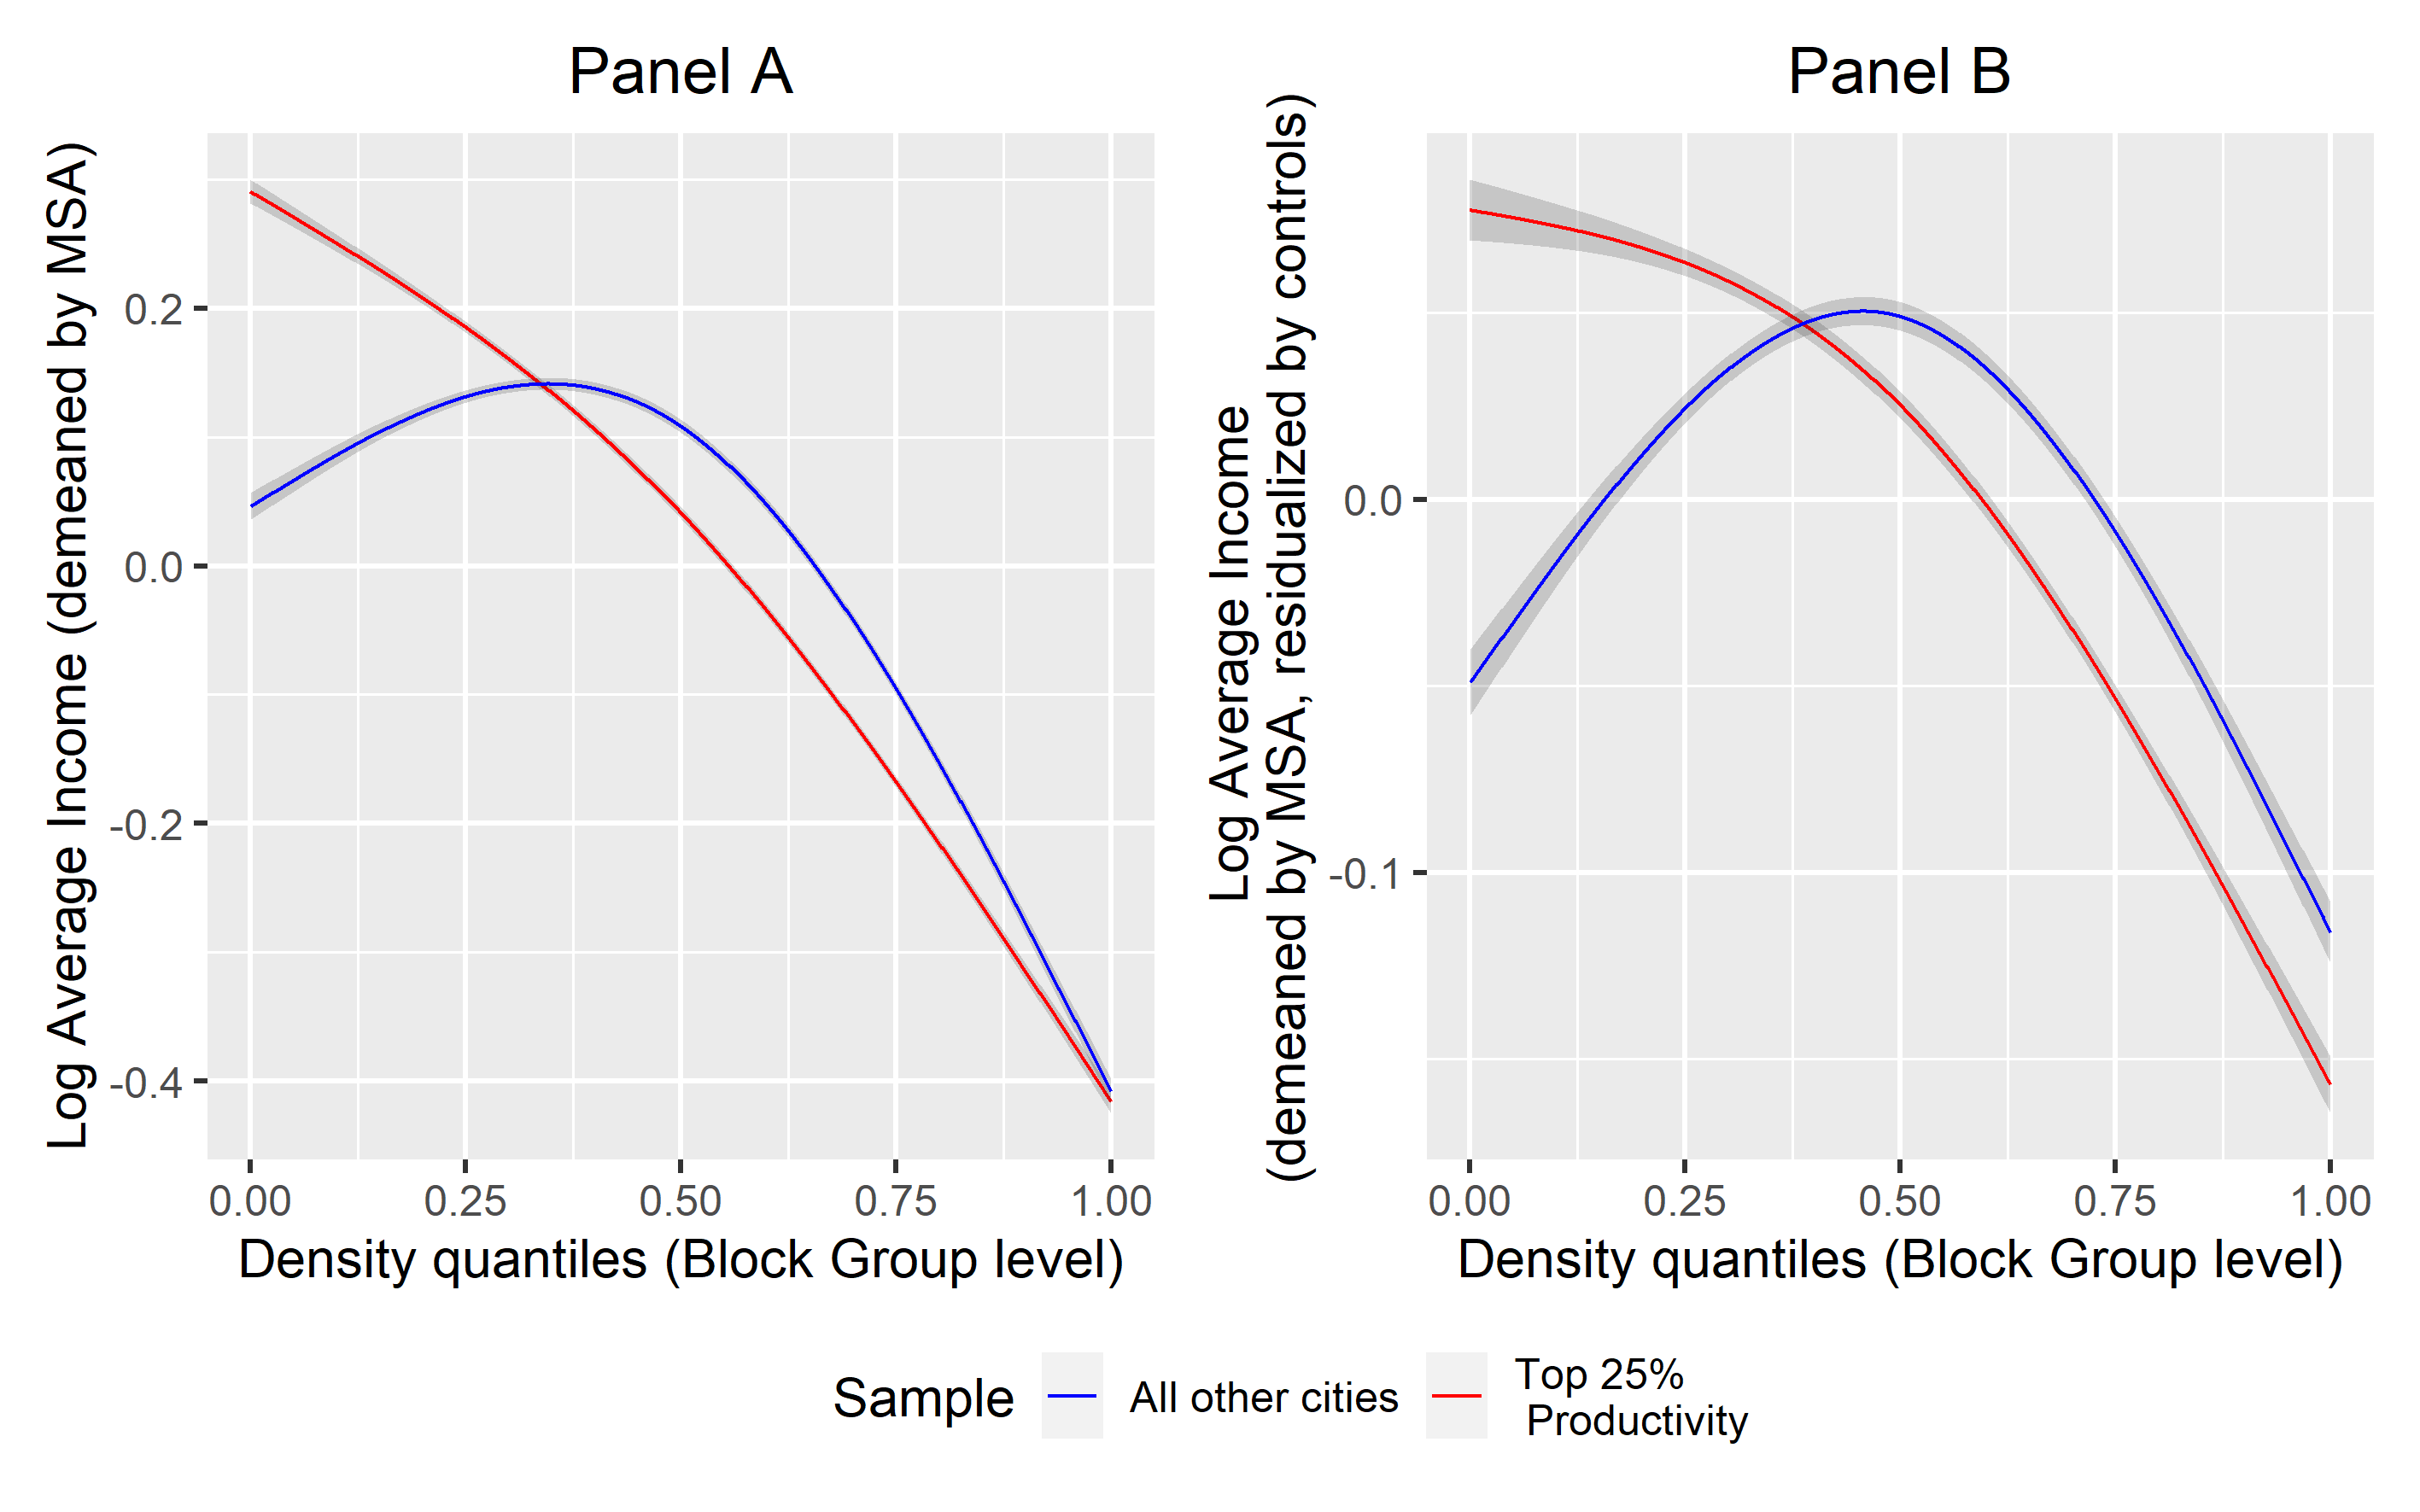
\includegraphics[width=\textwidth]{income_combined.png}
			\caption{Plot of cublic spline $\mathbf{S}$ from Equation \eqref{Specification:IncomeSortingStrong} with 5 knots, estimated with the \textit{mgcv} package in R \citep{gampackage}. 95\% confidence sets are reported. Panel A reports the model with  controls, while Panel B includes the model with the full set. The full set of controls are CBD distance, building age, household size, share of households using public transport to commute, share of households using cars to commute, and average commuting time time from the ACS; density of performing arts, spectator sports, casinos, recreational activities, restaurants, fast food, bars and coffee shop establishments from NaNDA; and the density of EPA toxic releases and the density of public transport stops from NaNDA. All variables from the ACS vary at the block group level, and at the tract level for NaNDA.  }\label{Figure:IncomeSortingStrong}
		\end{center}
	\end{figure}

	\paragraph*{}
	Panel A of Figure \ref{Figure:IncomeSortingStrong} reports $\mathbf{S}$ for superstar cities (in blue) and non-superstar cities (in red) with excluded controls. There is a clear negative relationship across samples for most points along the density distribution. There is also a significant difference in the income-density gradient; we see that the high density neighborhoods in dense cities are relatively less affluent, with the exception of block groups in the top 10 \% of the density distribution. Visually, this corresponds to the blue curve being below the red curve for most neighborhoods the top half of the density distribution. The pattern becomes even more stark in Panel B after accounting for other observable characteristics of these neighborhoods that cause income sorting. Panel B also shows that the differences in the gradients are large. For example, a neighborhood that is equivalent on observables in the $75$th percentile of the density distribution would be roughly $10$\% poorer relative to the mean in dense cities, and similarly $7.5$\% richer relative to the mean for neighborhoods in the $25$th percentile. 

	\paragraph*{} 
	Clearly, there must be some other mechanism that both correlates with density and drives income sorting that was not accounted for. This mechanism must also act differently in the largest cities in order to rationalize differences in the income-density gradients. It has long been argued that productive cities are more likely to impose stringent regulation \citep{HILBER2013,parkho, durantonpugaurbgrowth}. I echo a similar message and make an additional argument: within-city variation in regulation across neighborhoods is fundamentally different in dense cities. I end with Fact \ref{FStringency}. 

	\begin{Fact}\label{FStringency}
		(The geography of minimum lot sizes)
		\begin{enumerate}
			\item  Low density neighborhoods in expensive cities exhibit relatively higher regulatory stringency than cheap cities. Conversely, high density neighborhoods in dense cities are relatively less stringent. This explains the stronger income-density gradient in expensive cities. 		
			\item  The stringency of lot size regulation is significantly higher in expensive cities. This explains some positive income sorting into these cites. 
		\end{enumerate}
	\end{Fact}
	
	\paragraph*{} 
	To show Fact \ref{FStringency}, I first propose an intuitive measure of regulatory stringency that has foundations in the forthcoming model. This measure relies on two simplifying assumptions. Suppose we have measured a minimum lot size $l_{ic}$ (in acres) in some neighborhood $i$, and suppose exactly one household must rent at least the amount of structure on that minimal lot to live in a regulated structure in that neighborhood\footnote{To allow for duplexes, triplexes and quadriplexes, I adjust the minimal lot size by the associated unit density restriction.}. Implicitly, this means that the minimum lot size is uniform in $i$. In addition, assume that structure is supplied at a rate proportional to the size of the lot within $i$, and that the rental rate for a unit of structure is also uniform within $i$ and roughly proportional to the market value of the house. I define the novel \textit{stringency of minimum lot size regulation} $I_{ic}$ as the value of structure on a minimal lot where
	\begin{equation}\label{observedStringency}
		I_{ic} = V_{ic}l_{ic}L^{R}_{ic}
	\end{equation}
	where $V_{ic}$ is the housing value per acre in neighborhood $i$ and city $c$ observed from the CoreLogic transactions data. $L^{R}_{ic}$ is the ACS fraction of households who live in \textit{regulated structures}, which I define as those between 1 and 4 housing units per parcel. I construct land values per acre using CoreLogic transactions and assessments; by dividing the median transaction value for structures with 1 to 4 housing units per lot with the housing-unit weighted average amount of land per housing unit in these structures. To construct these land values, I exclude condominiums as it is often difficult to infer the number of housing units per parcel. Under the assumption that all other structure types do not face any regulatory constraints, $I_{ic}$ can be interpreted as the expected value of a minimal lot faced by a randomly selected household in $(i, c)$. In the model, higher stringency levels imply stronger income sorting -- households with low income are forced to spend a fraction of their income to rent the minimal lot beyond what they would if they could choose their housing consumption freely. 
	
	\paragraph*{}
	The first part of Fact \ref{FStringency} says that the stronger income-density gradient in expensive cities is met with a similarly stronger stringency-density gradient, suggesting that regulation is an underlying explanation. To show this, I alter the regression in Equation \eqref{Specification:IncomeSortingStrong} such that the dependent variable is instead $I_{i}$ demeaned by the average in $c$. The objective is essentially the same as in the exercise in Panel A of Figure \ref{Figure:IncomeSortingStrong}: to plot the function $\mathbf{S}$ associated with this regression for both city samples and compare them. I do so in Panel A of Figure \ref{Figure:StringencyStrong}, with controls excluded. 
	
	\begin{figure}[!ht]
		\begin{center}
			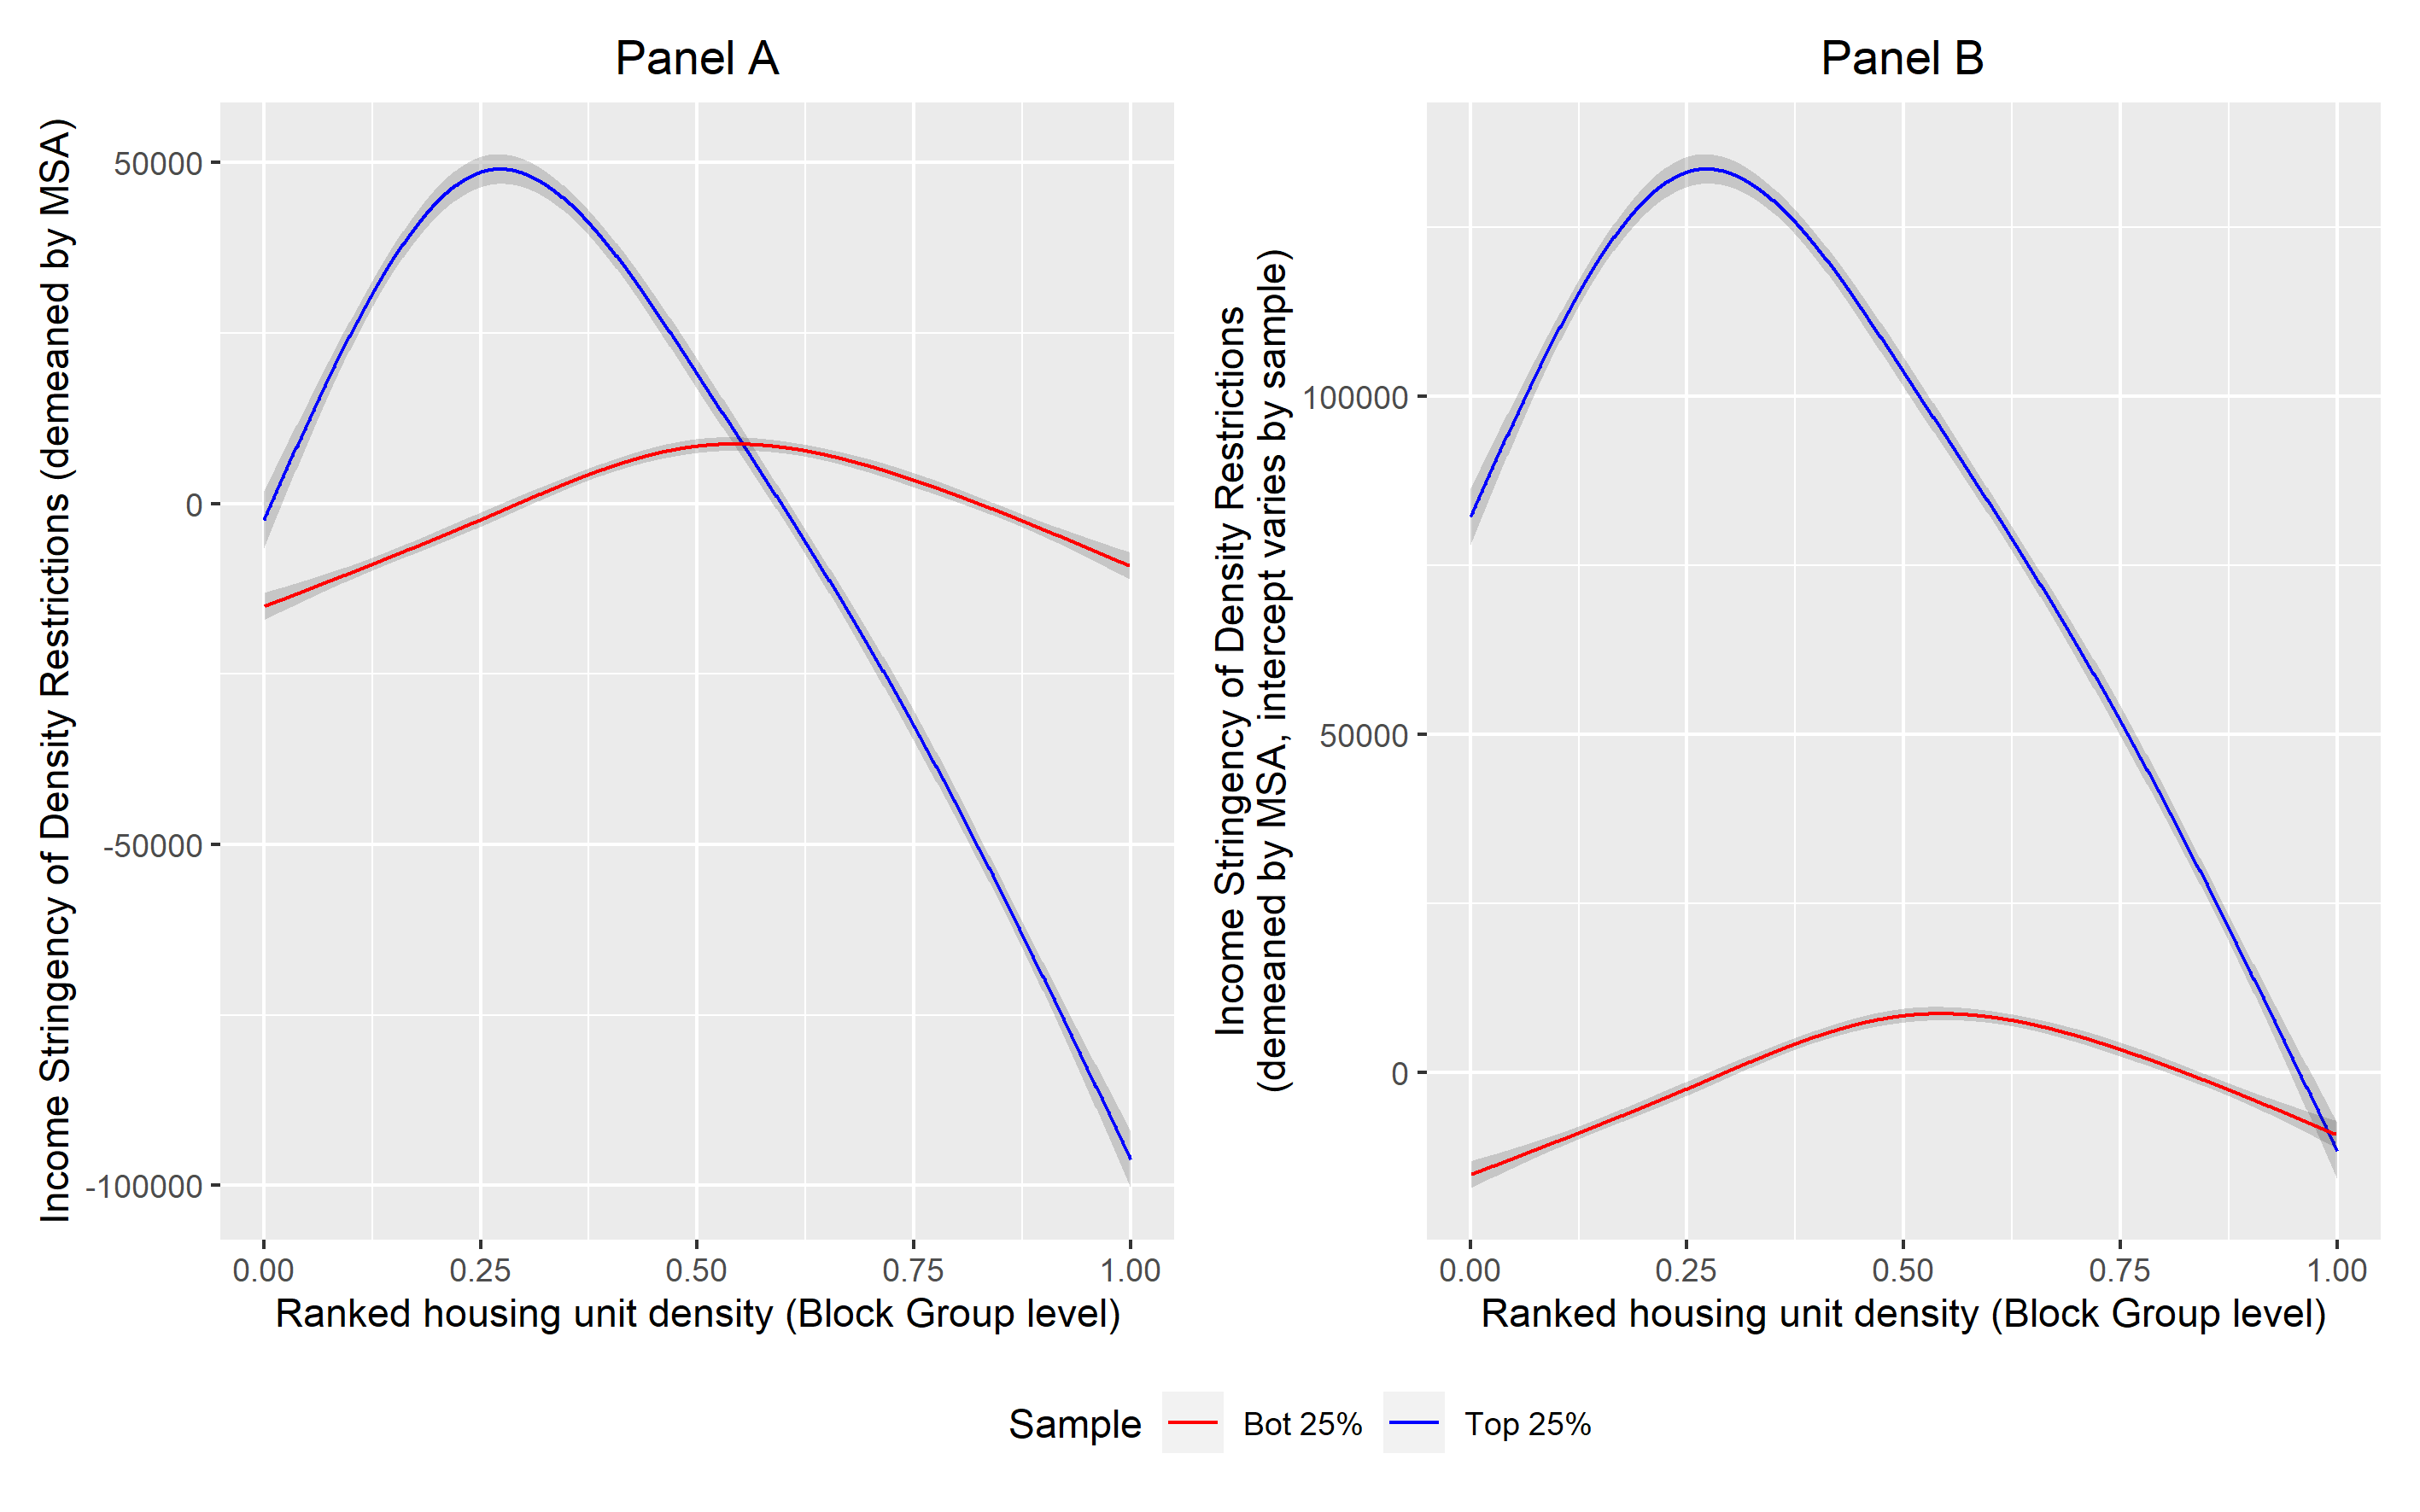
\includegraphics[width=\textwidth]{incomestringency_combined.png}
			\caption{Plot of cublic spline $\mathbf{S}$ with 5 knots, estimated with the \textit{mgcv} package in R \citep{gampackage}. The specification in Panel A replaces log income in Equation \eqref{Specification:IncomeSortingStrong} with regulatory stringency in Equation \eqref{observedStringency} and \textit{excluded} controls, demeaned by city and measured in 2012 US dollars. The residualized version of this regression (mirroring Panel B of Figure \ref{Figure:IncomeSortingStrong}) is omitted as they look qualitatively identical. 95 \% confidence sets are reported. Panel B repeats the same regression while allowing the average stringency to vary by sample. In other words, the blue curve is shifted upward by a constant. }\label{Figure:StringencyStrong} 
		\end{center}
	\end{figure}

	\paragraph*{}
	Panel A of Figure \ref{Figure:StringencyStrong} reveals a strikingly similar pattern to Panel B of Figure \ref{Figure:IncomeSortingStrong}: high density neighborhoods in expensive cities exhibit relatively less stringency, and low density neighborhoods relatively higher stringency. A qualitatively similar pattern holds when conditioning on controls, so the associated plot is omitted. These differences are large. The highest density neighborhood in a expensive city has the value of a minimal lot that is almost $\$ 150,000$ lower relative to the city mean. At the 25th percentile, expensive cities have a value that is roughly $\$ 25,000$ greater. These differences represent a significant proportion of the average value of a home, especially in high density neighborhoods. Conceptually, the differences in relative stringency at different points along the density distribution accompany differences in the \textit{types} of residential structures that appear. Think about the densest neighborhood in Los Angeles -- most of the housing units are in large multifamily structures, where there is no concept of a minimum lot size\footnote{Regulatory authorities could impose minimum floorspace requirements for units in large residential structures. However, these units tend to be consistently smaller than single family homes.}. Contrast this with a low density city like Abilene in Texas, where the densest neighborhoods consist of marginally smaller single family homes. 
	
	\paragraph*{}
	The second part of Fact \ref{Figure:StringencyStrong} says that expensive cities have higher levels of stringency in an average neighborhood. This observation can explain some income sorting into dense cities to the extent that this reflects sorting on skills or other household attributes \citep{diamond2016, citysizewagegap}. In Panel B of Figure \ref{Figure:StringencyStrong}, I show this by repeating the same regression as in Panel A while allowing the average stringency across neighborhoods to vary across the two samples. The figure shows that, in practically every neighborhood, average stringency levels are higher in dense cities. A typical neighborhood in the middle of the density distribution has a price of a minimal lot approximately $\$300,000$ greater in expensive cities. This gap in stringency does not disappear at any point along the neighborhood density distribution.
	\paragraph*{}
	It may be unsurprising that dense cities have more expensive minimal lots. However, the measure $I_{ic}$ is the product of two forces in Equation \eqref{observedStringency} -- while expensive cities naturally have higher housing prices per acre, they also tend to have smaller minimum lot sizes. The gap between the value per acre and the minimum lot size in productive cities reflect political economy forces; these arise endogenously in certain models of housing regulation, such as \cite{parkho} or \cite{HILBER2013}. Interestingly, these models cannot explain the stringency-density gradient within expensive cities, as they would predict neighborhoods with the best commuter accessibility to productive employment centers to have the highest level of regulation. While the objective of this paper is not to justify an alternative explanation, I can speculate. In the neighborhoods to allow for high density structures (like in high density neighborhoods in dense cities), the power for local homeowners to limit density is low. It may be because these neighborhoods are not fiscally decentralized\footnote{For example, San Francisco has one board responsible for city planning in the entire county. When approving projects, they commonly express interest in the welfare of renters, not just homeowners. The same might not be said for other neighboring jurisdictions like Palo Alto. A related idea is that downtowns are poor because the rich like to escape redistributive policies, as hypothesized in \cite{NechybaWalsh}.}, and this matters for stringency insofar as it is a tool to create efficient Tiebout sorting \citep{calabresetal}. It may also be because these neighborhoods predate the enforcement of regulation and where "locked in" to high density\footnote{I thank Will Strange for this suggestion.}. Whatever it may be, the purpose of this paper is to show why this variation in regulation matters for policy. I do so below. 
	
	
	\paragraph*{Implications for deregulation} Facts \ref{FIncomeDens} and \ref{FStringency} inform how large scale deregulation might affect the welfare of spatially mobile households. The macroeconomic literature emphasizes that housing regulation limits aggregate labour productivity because it limits the size of productive cities. This assertion is muddied by the fact that labour supply to any given city depends both on the number of households and the labour supply per household. If regulation causes productive cities to have a high labour supply per household as suggested by Fact \ref{FStringency}, then any productivity gains from deregulation could be offset by the out-migration of affluent households. Indeed, eliminating all minimum lot sizes in the forthcoming model finds gains to aggregate labour productivity of about $0.5 \%$, which is more than 10 times smaller than the outcomes of similar exercises, in particular that of \cite{hseihmoretti} and \cite{durantonpugaurbgrowth}.  
	
	\paragraph*{}
	On the other hand, within-city variation in income and lot size stringency highlighted in Facts \ref{FIncomeDens} and \ref{FStringency} suggest a correlation between neighborhood income and regulatory stringency along the urban density gradient, particularly in expensive cities. This is important if the sorting of high income households are associated with positive externalities. I argue in the following section that if income sorting that would occur in the absence of this regulation were strong, then imposing stringent regulation in high income neighborhoods can correct an externality associated with demand spillovers caused by high income neighbors\footnote{In other words, the imposition of minimum lot sizes in rich neighborhoods would cause reallocations of the lowest income households in rich neighborhoods to become the highest income households in poor neighborhoods; increasing average income everywhere. I show that this reallocation is a Pareto improvement for renters with a simple model in Section \ref{Section:Model}.}. If such strong income sorting characterizes the world be observe, then these facts suggest that low density neighborhoods in expensive cites are rightfully imposing more stringent regulation. On the other hand, if the income density gradient we observe in Fact \ref{FIncomeDens} would be much flatter in the absence of regulation (in other words, if income sorting in the absence of regulation is weak), I show that stringent minimum lot sizes cause largely distributional consequences, benefiting high income households necessarily at the expense of lower income households. An important consequence of the latter scenario is that deregulation will cause initially poor neighborhoods to gentrify, decreasing residential income segregation overall. Facts \ref{FIncomeDens} and \ref{FStringency} suggest that the poorer neighborhoods are precisely the higher density neighborhoods of expensive cities. Model counterfactuals in Section \ref{Section:Counterfactuals} predict these gentrification patterns.
	
	\paragraph*{Robustness}
	Before continuing to the model, I note that there are many arbitrary choices used to construct the data to generate these facts. In Appendix \ref{Appendix:Robustness}, I show that the facts are robust to alternative weights, clustering schemes, definitions of superstar cities, and various combinations of control variables and time periods. I also discuss instances where the facts do not hold, namely when replacing the use of density rankings with distances to the central business district.  
	
	
%__________________________________________________________________________
\section{Theoretical framework}\label{Section:Model}
%__________________________________________________________________________	
	
	\paragraph*{}
	In this section, I introduce a simple quantitative framework that can be taken to the data to assess the consequences of deregulation, particularly the relative importance of its effect on housing affordability, aggregate labour productivity, and the external costs associated with neighborhood choice. I analyze a few simple cases of the model and provide two broad messages. First, the model can qualitatively rationalize Facts \ref{FIncomeDens} and \ref{FStringency} with little structure. Second, I show minimum lot sizes are Pareto improving when income sorting is strong in the absence of regulation; I also show that minimum lot sizes cause largely distributional consequences when income sorting is instead weak. The full quantitative framework is designed to be able to match any arbitrary pattern of observed income sorting and nests both of these quantitative predictions that the data can speak to.  
	
	\subsection{The Quantitative Spatial Model}
	
	\paragraph*{Geography}
	I consider a finite set of cities $\mathbb{C}$ indexed by $c$, which map to MSAs in the data. These cities are self-contained labour markets; that is, I do not allow households to access productive technologies outside of the city for which they reside. Each city $c$ has an exogenous finite set of neighborhoods $N(c)$. I use the index $i$ to denote a typical neighborhood from any city, $i \in \cup_{c \in \mathbb{C}}N(c)$, and define the map $\mathbb{C}(i)$ to be the city associated with $i$. Neighborhoods are 2020-definition census block groups. Each of these neighborhoods have an exogenous amount of land $T^{R}(i)$ zoned for \textit{regulated structures} and land $T^{U}(i)$ zoned for any type of structure. Like in the empirical work, regulated structures are those with between 1-4 housing units per parcel. I use the notation $\boldsymbol{o} \in \{R, U\}$ to index unregulated and regulated zones, respectively. Land in each zone will be calibrated to target the observed share of households who reside in regulated structures in each neighborhood. This distinction is important, as high density locations (like downtown New York City) appear to have expensive single family homes but a disproportionately small share of units that comprise them.

	\paragraph*{Housing Developers}   
	In anticipation of households making choices over neighborhoods to reside, I assume that exactly one household can occupy one housing unit. In a standard model of housing supply, developers are indifferent to producing any number of housing units\footnote{See, for example, the housing supply model in \cite{BSH}.}. This means that the number of housing units can be arbitrarily large; as large as the number of households who choose the neighborhood in equilibrium. Complicating this problem is the \textit{minimum lot size} $\bar{l}(i)$ and the regulation of how many housing units can occupy each lot. To make the exposition clear, I start with preliminaries. In each neighborhood, I partition residential land in regulated structures $T^{R}(i)$ into equal sized \textit{parcels} of normalized mass $1$. That is, there are a mass $T^{R}(i)$ of parcels. These are the units of land that the representative developer uses to produce structure. These parcels can be \textit{split} or \textit{combined} into lots, and lots are a fundamental unit by which regulation operates. Each lot can hold a regulated maximum $\bar{h}(i)$ housing units. For example, $i$ may allow duplexes, so that $\bar{h}(i) = 2$. Then, $\bar{l}(i)/\bar{h}(i)$ is the minimum amount of land per housing unit in $i$. Let $l(i)$ denote this minimum land per housing unit, which will be the main object I work with hereafter\footnote{An implicit assumption is that there is no material difference between single family homes on small lots or multifamily homes on large lots. This is obviously untrue if households have lower demand for multifamily units, all else equal. I control for these implicit quality differences using a hedonic regression introduced in Section \ref{Section:CalibrationEstimation}.}. $l(i)$ may be zero if the neighborhood is unregulated. $l(i)$ is constructed from lot size data using the procedure in Section \ref{Section:Evidence}. 

	\paragraph*{}
	Given a parcel in $i$, developers choose the total amount of structure $A(i)$ that occupy it in a standard way. That is, they use a neighborhood-varying Cobb-Douglas technology over land and capital, facing a perfectly elastic supply of that capital at rate $r$. This yields the neighborhood-zone level housing supply function per unit of land
	\begin{equation}\label{supplyfn}
		A_{\boldsymbol{o}}(i) = \lambda(i)P_{\boldsymbol{o}}(i)^{\epsilon(i)}
	\end{equation}
	where $P_{\boldsymbol{o}}(i)$ is the price of a unit of housing stock in zone $\boldsymbol{o}$, $\epsilon(i)$ is the supply elasticity and $\lambda(i)$ is an exogenous supply shifter. In a world without minimum lot sizes, the developer is indifferent to allocating this structure across housing units; there can be many small houses or few large ones, provided the total stock is given by \eqref{supplyfn}. Instead, if developer in zone $R$ respect the minimum lot size, the minimum amount of housing stock per housing unit $A^{\star}(i)$ must be

	\begin{equation}\label{minstructure}
		A^{\star}(i) = \lambda(i)P_{R}(i)^{\epsilon(i)}l(i)
	\end{equation}

	\paragraph*{}
	I take the quantity $A^{\star}(i)$ as a minimum amount of housing services required to be purchased to live in a regulated structure in neighborhood $i$. Define the quantity 
	
	\begin{equation}\label{stringency}
		I(i) = P_{R}(i)A^{\star}(i).
	\end{equation}
	$I(i)$ is the cost to rent housing services on a minimal lot in the regulated zone. This is the model equivalent to the observed stringency of regulation in Equation \eqref{observedStringency} used to construct Fact \ref{FStringency}. Households with little disposable income after paying for this minimum quantity are forced to purchase more than what they would if this quantity could be freely chosen. This arises naturally from the household's consumption problem. In the unregulated zone $U$, I assume there is no minimum lot size, and this is equivalent to assuming $l(i) = 0$. 
	
	\paragraph*{}
	Equation \eqref{minstructure} reveals the material difference between lot size regulation and other regulations studied in contemporary quantitative models. Contrast the equation with the standard Floor Area Ratio restriction in \cite{bruecknersingh}, which puts limits on the density of floorspace in each parcel. Here, there are no such limits. Instead,  on the number of housing units (or households) that can occupy a parcel. This distinction is forcefully argued in \cite{griesonwhite}. Most work studying the aggregate implications of housing regulation \textit{assume} that regulation affects the supply elasticity $\epsilon(i)$ or productivity $\lambda(i)$, amounting to regulation on the density of floorspace \citep{hseihmoretti, parkho, hop}. In this paper, minimum lot sizes do nothing except block the supply of low quality housing units, leaving $\epsilon(i)$ and $\lambda(i)$ unchanged.  

	
	\paragraph*{Household Consumption}
	Households have Stone-Geary preferences over a freely traded, homogenous good $g$ (with a normalized price of 1 dollar) and housing services $A$. Households differ on \textit{income type} indexed by $z \in Z$, where $Z$ is finite, and hold no land wealth. Alternatively, $z$ is the labour supply of the household. Let $\bar{L}(z)$ be the mass of type $z$ households. Deferring location choice for a moment, suppose a household of type $z$ has chosen neighborhood $i$ and zone $\boldsymbol{o}$. Given the city $\mathbb{C}(i)$, households receive a wage $w(\mathbb{C}(i)) := w(i)$ per effective unit. Given this wage, the household of type $z$ chooses consumption $g$ and housing services $A$ to maximize
	\begin{equation}\label{utility}
	\max_{A, g} \beta^{-\beta}(1-\beta)^{-(1-\beta)}(A - \bar{A})^{\beta}g^{1-\beta}
	\end{equation} 
	subject to $P_{\boldsymbol{o}}(i)A \geq I(i)$ if $\boldsymbol{o} = R$, and $P_{\boldsymbol{o}}(i)A + g \leq w(i)z$, where $\bar{A}$ is a minimum level of housing services that must be consumed. Let  $V_{\boldsymbol{o}}(i, z)$ be the solution to Problem \eqref{utility}, which implicitly depends on prices in each zone, wages and other endogenous variables. If a consumer chooses a minimally sized lot whose price exceeds income at $z$, I set  $V_{\boldsymbol{o}}(i, z) = 0$ and assume that the household spends all their income on housing. Similarly, I set $V_{\boldsymbol{o}}(i, z) = 0$ if a household cannot afford $\bar{A}$ units of housing services in $i$ irrespective of regulation. To see how regulation in zone $R$ distorts housing consumption, $V_{R}(i, z)$ can be decomposed into two components when preferences are Cobb-Douglas ($\bar{A} = 0$) and the minimum lot size is binding:
	
	\begin{equation}\label{utilitydecomp}
		V_{R}(i, z) = \underbrace{\frac{w(i)z}{P_{R}(i)^{\beta}}}_{\text{Undistorted utility}}  \times \underbrace{\bigg[\frac{\beta}{\frac{I(i)}{w(i)z}}\bigg]^{\beta}\bigg[\frac{1 - \beta}{ 1- \frac{I(i)}{w(i)z}}\bigg]^{1 - \beta}}_{\text{Distortion factor}}
	\end{equation}
	whenever $\beta w(i)z < I(i)$, so that the desired spending on housing is smaller than the cost to rent a minimal lot. The distortion factor is 1 when the minimum lot size is nonbinding, and is decreasing in the distance between the desired spending share on housing $\beta$ and the spending share on housing $\frac{I(i)}{w(i)z}$ induced by regulation. An immediate consequence of \eqref{utilitydecomp} is that the disutility of regulation is decreasing in income $z$, or 
	
	\begin{equation}\label{supermodularity}
	\frac{\partial V_{R}(i, z)}{\partial I(i) \partial z} > 0 	
	\end{equation} 
	 all else equal, whenever $\bar{A} = 0$ and regulation is binding at $z$. 

	\paragraph*{Zone choice}
	I assume households are perfectly mobile across zones. In other words, households choose zones to solve 
	
	\begin{equation}\label{zonechoice}
		V(i, z) := \max_{\boldsymbol{o} \in \{R, U\}}V_{\boldsymbol{o}}(i, z)
	\end{equation}
	When choosing zones within a neighborhood, there is an implicit trade off that varies across income types. To make this trade off as clear as possible, first note that higher minimum lot sizes in the model strictly decrease utility, all else equal. This is because, at best, they do not bind housing consumption decisions, and at worst make housing consumption too large. If prices per unit of housing services were equal across zones, this means that nobody would choose the regulated one. In spatial equilibrium, the disutility of a large lot must be compensated by a relatively lower price per unit of housing services in the regulated zone. However, this logic will \textit{not} hold when making comparisons of regulation across neighborhoods. This is because neighborhood amenities will endogenously respond to the level of regulation, and I introduce that portion of the model later in the section. 

	\paragraph*{Neighborhood choice} 
	Apart from consumption of housing and other goods, each neighborhood $i$ provides an \textit{amenity value} $b(i, z)$ for households of observed type $z$. Crucially, amenities $b(i, z)$ are flexible enough to rationalize any local population and income distributions across neighborhoods that may be observed. The structure of these amenities will imply a rich set of counterfactual predictions of deregulation, as I show at the end of this section. Along with these amenities, households draw idiosyncratic amenities shocks over neighborhoods, and these shocks are distributed Gumbel. The mass of $z$ households who choose neighborhood $i$ is 
	\begin{equation}\label{laboursupply}
	L(i, z) = \bigg[\frac{W(C(i), z)}{\boldsymbol{W}(z)}\bigg]^{\theta}\bigg[\frac{e^{V(i, z)}b(i, z)}{W(\mathbb{C}(i), z)}\bigg]^{\rho}\bar{L}(z)
	\end{equation}
	where
	\begin{equation*}
	W(\mathbb{C}(i), z) = \bigg[\sum_{i' \in N(\mathbb{C}(i))}\big[e^{V(i', z)}b(i', z)\big]^{\rho}\bigg]^{\frac{1}{\rho}}
	\end{equation*} 
	is the expected welfare of a household $z$ who chose a neighborhood in $\mathbb{C}(i)$ and 
	\begin{equation}\label{Welfare}
		\boldsymbol{W}(z) = \bigg[\sum_{c \in \mathbb{C}} W(c, z)^{\theta}\bigg]^{\frac{1}{\theta}}	
	\end{equation}
	is the expected welfare of a type $z$ household before drawing a shock.  This is our standard measure of renter welfare moving forward. $\theta$ governs how responsive migration flows are to changes in neighborhood valuations. $\rho$ governs the responsiveness of migration flows across neighborhoods within a given city. 
 
	\paragraph*{Amenities} So far, regulation is a disamenity because it constrains the housing consumption possibilities of certain households. This is not true when neighborhood quality responds endogenously to regulation. I assume that amenity values $b(i, z)$ depend on the average income of a neighborhood
	\begin{equation}\label{endoamen}
		\log\big[b(i, z)\big] = \Omega(z)\log\bigg[\frac{\sum_{z' \in Z}w(i)z'L(i', z')}{\sum_{z' \in Z}L(i', z')}\bigg] + \log \nu(i, z)
	\end{equation}
	 The first term on the right hand side is income per capita of neighborhood $i$. I call $\nu(i, z)$ \textit{fundamental amenities}, which contain all other observed or unobserved factors that determine amenity values that can be reasonably taken as exogenous with respect to this model, such as commuting infrastructure or natural amenities. $\Omega(z)$ will be estimated using a donut strategy in Section \ref{Section:CalibrationEstimation}. 

	 \paragraph*{}
	There are at least two main channels that I have emphasized thus far that would proximally give rise to \eqref{endoamen}. Firstly, local income could increase local amenities through variety effects in a Dixit-Stigliz style model \citep{AlmagroDI, Coutureetal}, while local population could decrease the amenity value through urban congestion effects or from the disutility of density highlighted in \citep{KSC}. When these two forces operate at the same elasticity $\Omega(z)$, amenity values depend only on income per capita. Secondly, local governments could provide a congested public good financed through income or property taxes \citep{calabresetal, ineffTiebout}. In the latter case, income per capita would be replaced with property tax revenue per capita. In a model with Cobb-Douglas preferences over housing, no minimum lot sizes and random heterogeneity in property tax rates, this essentially identical to income per capita. With Stone-Geary preferences and minimum lot sizes, the relationship between property tax revenue and incomes need not be linear, but nevertheless they would still be highly correlated. In Appendix \ref{microfoundations}, I provide microfoundations for each of these mechanisms. However, I do not want to limit myself to them. Instead, I assume $\Omega(z)$ reflects all factors that could be \textit{caused} by the compositional effects of affluence. Apart from the above, these may include reduced crime, peer effects \citep{chettyhendren}, or a general taste for affluent neighbors \citep{ghh2013, parispoor}. Finally, I close the model by specifying how wages are determined.

	\paragraph*{Production} In each city $c$, production of the numeraire good $g$ takes place competitively at a central business district with a constant-returns technology
	\begin{equation}\label{production}
		g(c) = \iota(c)\bigg[\sum_{i \in N(c)}\sum_{z \in Z}zL(i, z)\bigg]
	\end{equation}
	where $\iota(c)$ is the exogenous labor productivity in city $c$. In equilibrium, it must be that $\iota(c) = w(c)$ and so I 	refer to both interchangeably. Aggregate labour productivity is thus 
	\begin{equation*}
		\frac{\sum_{c \in C}g(c)}{\bar{L}}
	\end{equation*}
	 where $\bar{L}$ is the total mass of households nationally. Differences in labor productivity and populations across cities will be crucial for understanding aggregate labour productivity, as in \cite{hseihmoretti}. Additionally, I argue that differences in the labour supply per household across cities matters when assessing the impacts of deregulation because this regulation cannot be decoupled from income sorting.
 
	\paragraph*{}
	 The production technology in Equation \eqref{production} is restrictive in two important ways. First, relative flows of high and low income workers alter the relative wage they earn if these workers are not perfect substitutes in production \citep{card}. Second, population flows across cities cause changes in labor productivity via agglomeration effects \citep{Combes_review}. Moreover, these agglomeration effects may be biased in their benefit to high income workers, as is suggested by evidence in \cite{diamond2016} and \cite{ineqincreased}. Since deregulation changes both the population and skill composition of cities, each of these mechanisms may be quantitatively important for the counterfactual. In Appendix (xx), I provide multiple extensions to the baseline technology \eqref{production} and discuss the implications of each for deregulation. The main message of this paper is robust to each of these extensions. 
 
	\paragraph*{}
	With housing and labour markets defined, I turn to the definition of an equilibrium.

	\paragraph*{Equilibrium} An equilibrium is defined as a set of housing prices $P_{\boldsymbol{o}}(i)$, neighborhood allocations $L(i, z)$, amenities $b(i, z)$ such that
	\begin{enumerate}
		\item Labour Markets clear: Given indirect utility $V(i, z)$ solving \eqref{utility}, amenities $b(i, z)$ solving \eqref{endoamen}, labour supply per household type $L(i, z)$ solves \eqref{laboursupply} at wages $w(c) = \iota(c)$.
	
		\item Housing Markets clear: Given $A^{\star}(i)$ solving \eqref{minstructure} and population $L(i, z)$, the neighborhood demand for housing stock derived from \eqref{utility} equals the neighborhood supply of housing stock derived from \eqref{supplyfn} in every $i$. 
	\end{enumerate}

	
\subsection{Replicating the facts with the model}\label{SubSection:ReplicatingFacts}
	\paragraph*{}
	Facts \ref{FIncomeDens} and \ref{FStringency} say that expensive cities are on average higher income and exhibit stronger negative income sorting on density, and that this can be explained by the spatial variation in the prices of minimal lots $I(i)$. With little structure on the model, I construct an equilibrium in which a chosen set of minimum lot sizes $l(i)$ reproduce both of these facts. 

	\paragraph*{}
	To make the example as simple as possible, I assume there are two cities: a superstar city $c_{1}$ and non-superstar $c_{0}$. There are two income types $z_{0}$ and $z_{1}$ with $z_{0} < z_{1}$. The \textit{only} difference between these two cities is productivity $\iota(c_{0}) < \iota(c_{1})$. Each city $c$ has two neighborhoods of unit land mass $i_{c0}$ and $i_{c1}$ where the minimum lot size in $i_{c1}$ is $\bar{l} > 0$ and the minimum lot size in $i_{c0}$ is 0, and each neighborhood offers identical fundamental amenity value $\nu(i, z)$ for both income types. I make no distinction between regulated and unregulated zones. Finally, I assume all neighborhood amenities are exogenous, $\Omega(z) = 0$ for all $z$, the migration elasticity across cities and neighborhoods is infinite, and preferences are homothetic, $\bar{A} = 0$.  
	\paragraph*{}
	 Neighborhoods $i_{c0}$ and $i_{c1}$ will be ordered by affluence and inversely ordered by density because of the variation in regulation between them. While both cities have the exact same variation in physical minimum lot sizes across neighborhoods, differences in the value of a minimal lot $P(i)A^{*}(i)$ will arise in equilibrium because city $c_{1}$ will have a higher value of land. This leads to the income sorting patterns observed in the data, as summarized in Proposition \ref{Prop:ReproduceFacts}.
	\begin{Proposition}\label{Prop:ReproduceFacts}
	Suppose $\bar{l}$ and relative productivity $\frac{\iota(c_{1})}{\iota(c_{0})}$ are sufficiently large. Then, the following hold in equilibrium:
	
		\begin{enumerate}
			\item City $c_{1}$ is relatively more affluent, $\frac{L(c_{1}, z_{1})}{L(c_{1}, z_{0})} > \frac{L(c_{0}, z_{1})}{L(c_{0}, z_{0})}$ where $L(c, z)$ is the city $c$ population of type $z$ households.
		
			\item In each city $c$, neighborhood $i_{c0}$ has a weakly higher density of housing units relative to $i_{c1}$. This inequality is strict in $c_{1}$. 
		
			\item City $c_{1}$ exhibits a stronger negative income-density gradient, $$\frac{L(i_{c_{1}1}, z_{1})}{L(i_{c_{1}0}, z_{1})}/\frac{L(i_{c_{1}1}, z_{0})}{L(i_{c_{1}0}, z_{0})} < \frac{L(i_{c_{0}1}, z_{1})}{L(i_{c_{0}0}, z_{1})}/\frac{L(i_{c_{0}1}, z_{0})}{L(i_{c_{0}0}, z_{0})} \leq 1$$ where $L(i_{c}, z)$ is the population of type $z$ households in neighborhood $i_{c}$. 
		\end{enumerate}
	
	\end{Proposition}
	\begin{proof}
		See Appendix \ref{Proof:ReproduceFacts}.
	\end{proof}
	\noindent The condition that relative productivity $\frac{\iota(c_{1})}{\iota(c_{0})} $ and the minimum lot size $\bar{l}$ is large ensures that the low density neighborhood in $c_{1}$ has a minimum lot size that is strictly binding for at least the lowest income group $z_{0}$. Under this parameterization of the model, there is purposefully no reason for income sorting across and within cities in the absence of minimum lot size regulation. This is because each location provides identical fundamental amenity value for households of all incomes\footnote{In addition to preferences being assumed homothetic to prove Propositon \ref{Prop:ReproduceFacts}.}. Consequently, each of the results in Proposition \ref{Prop:ReproduceFacts} are causal effects of regulation, rather than some other artifact of the model.
	
\subsection{When does regulation benefit all renters?}\label{Theory:Externality}

	\paragraph*{}
	Under the model structure assumed in Proposition \ref{Prop:ReproduceFacts}, all income segregation across neighborhoods and cities is induced only by regulation. The regulated, high income neighborhood in the productive city $i_{c1}$ offers cheaper prices per unit of housing services to compensate for the fact that too much housing services need to be purchased to live there\footnote{Or, in the full model, these neighborhoods could offer higher amenities as another compensating differential.}. Additional inequality between the two income types is induced by the creation of this high value neighborhood. In other words, regulation causes mostly distributional consequences, so that the value of the policy depends solely on how much weight high income households are given in the social welfare function. In this section, I contrast this regressive outcome with another parameterization of the model; one where a specific structure of minimum lot sizes lead to Pareto improvements for every renter when amenities are endogenous. Pareto improvements are achieved by reallocating the poorest households in rich neighborhoods to become the richest households of poor neighborhoods, increasing amenity values everywhere. This result depends crucially on the structure of income sorting in the absence of regulation, which is governed by the fundamental amenities $\nu(i, z)$\footnote{The idea that income sorting creates an externality by which too many lower income households crowd rich neighborhoods has previously been used to argue that fiscal centralization across neighborhoods is typically more efficient than decentralization \citep{ineffTiebout}. The reasoning behind this argument is the same reasoning I use here.}. 
		
	\paragraph*{}
	To show this, I impose the following changes to the model parameterization used in Section \ref{SubSection:ReplicatingFacts}. Suppose there is instead three income types $z_{l} < z_{m} < z_{h}$ (low, medium and high), one city and two neighborhoods $i_{0}$ and $i_{1}$. These neighborhoods will be ordered in equilibrium by affluence because of both variation in regulation and additional income sorting induced by the fundamental amenities $\nu(i, z)$. In particular, I assume 
	
	\begin{eqnarray*}
		\nu(i_{0}, z_{l})  = \nu , & \nu(i_{1}, z_{l}) = 0 \\
		\nu(i_{0}, z_{m})  = \nu & \nu(i_{1}, z_{m})  = \nu \\ 
		\nu(i_{0}, z_{h})  = 0 & \nu(i_{1}, z_{h})  = \nu
	\end{eqnarray*}
	for any $\nu > 0$. The spatial distribution of these amenities implies strong income sorting on income in the absence of regulation. This is because the low income type $z_{l}$ will only sort into the less affluent neighborhood $i_{0}$ and conversely the high income type $z_{h}$ will only sort into $i_{1}$. Lastly, I assume that amenities are endogenous but $\Omega(z)$ does not vary by income type $z$. 
	\paragraph*{}
	Under these assumptions, I propose a distribution of minimum lot sizes $l(i)$ corresponding to an equilibrium that Pareto dominates the unique unregulated equilibrium for renters. In the unregulated equilibrium, too many middle income types sort into the affluent neighborhood $i_{1}$ because these neighborhoods provide a higher amenity value. This additional sorting of middle income types brings down the average income in \textit{both} neighborhoods and thus their amenity value. This cost is not internalized by the medium income types when they make these location decisions. To understand why using minimum lot sizes to reverse this "additional" sorting is Pareto improving for renters, consider how households of each income type benefit. High income renters appreciate higher amenities and lower rents because there are less middle income types to bring down average income and congest housing markets. Low income renters appreciate this reallocation if the value of increasing amenities dominates the accompanying disutility of an increase in rents, which requires that housing supply is moderately elastic or housing consumption is given a low weight in the utility function relative to $\Omega$. Lastly, the value of the policy to middle income types is not obvious, as some of them are necessarily excluded from the affluent neighborhood. The logic here is that, in the unregulated spatial equilibrium, both neighborhoods provide identical value to the middle income types. If regulation that causes a reallocation of these types to the poorer neighborhood $i_{0}$ and that increases the utility value of the neighborhood for middle income types who originally live in $i_{0}$, then this must mean that utility increases for this income type in general. This logic is detailed in the proof of Proposition \ref{Prop:NeighborhoodChoiceExt}. 
	
	\begin{Proposition}\label{Prop:NeighborhoodChoiceExt}
		Suppose the structure of fundamental amenities $\nu(i, z)$ as above and $\Omega(z) = \Omega$ for some $\Omega > 0$. Moreover, $\beta$ is the Cobb-Douglas weight on housing consumption and $\epsilon$ is the housing supply elasticity in each neighborhood. Then,
		
		\begin{enumerate}
			\item The unregulated equilibrium is unique, and 
			
			\item From a unique unregulated equilibrium such that $L(i, z_{m}) > 0$ for all $i$, imposing a marginal increase in the lot size $l$ in $i_{1}$ such that it is binding only for type $z_{m}$ causes a Pareto improvement for all renters if and only if $$k \Omega > \frac{\beta}{1 + \epsilon}$$ for some $k > 0$. 
		\end{enumerate}
	\end{Proposition}
	
	\begin{proof}
		See Appendix \ref{Proof:NeighborhoodChoiceExt}.
	\end{proof}
	\noindent The condition $k \Omega > \frac{\beta}{1 + \epsilon}$ for some $k > 0$ expresses the trade off between higher amenities and higher rents when reallocating middle income types toward the poor neighborhood $i_{0}$. 
	
	\paragraph*{}
	Income sorting caused by variation in fundamental amenities $v(i, z)$ is crucial to facilitate these Pareto improvements. To show this, I contrast with outcome of Proposition \ref{Prop:NeighborhoodChoiceExt} with an equilibrium that exhibits no income sorting in the absence of minimum lot sizes. In this environment, there is no scope for regulation to correct the externality created by too many middle income types crowding in rich neighborhoods precisely because each neighborhood is identical in the absence of regulation. Imposing regulation in one neighborhood from this equilibrium decreases welfare for low income households by excluding them from neighborhoods with higher amenity value and lower prices per unit of housing services. This leads to Proposition \ref{Prop:NeighborhoodChoiceExt2}.
	
	\begin{Proposition}\label{Prop:NeighborhoodChoiceExt2} 
		
		
		Assume the same model structure used in Proposition \ref{Prop:NeighborhoodChoiceExt} with the exception that $\nu(i, z) = \nu$ for every $i$ and $z$, and for some $\nu > 0$. Then, 
		
		\begin{enumerate}
			\item When all neighborhoods are unregulated, there exists a symmetric equilibrium and
			
			\item If high income households take up a relatively small share of the population and their income is large, then there exists a set of minimum lot sizes imposed in $i_{1}$ such that
			
			\begin{enumerate}
				\item $i_{1}$ has higher income and lower rents relative to the symmetric equilibrium; the opposite is true for $i_{0}$.
				\item  $z_{h}$ types benefit and all other types lose relative to the symmetric equilibrium.
			\end{enumerate}	
		\end{enumerate}
	\end{Proposition}
	
	\begin{proof}
		See Appendix \ref{Proof:NeighborhoodChoiceExt2}.
	\end{proof}
	

	
	\paragraph*{}
	Propositions \ref{Prop:NeighborhoodChoiceExt} and \ref{Prop:NeighborhoodChoiceExt2} suggest that different parameterizations of the model have different distributional consequences. They also hint at different welfare implications for the average household if there are relatively many lower income households. An important question is which, if any, of these examples better characterizes the actual world we live in. A contribution of this paper is to have a model that can nest these competing hypotheses. In the deregulation exercise of Section \ref{Section:Counterfactuals}, I find that the contribution of the neighborhood choice externality to overall welfare is minimal for the average household, but has important distributional consequences. This suggests that the data is better described by little income sorting absent regulation as in Proposition \ref{Prop:NeighborhoodChoiceExt2}. This is also commensurate with the idea that minimum lot sizes drive a large portion of income sorting on density within and across cities (Facts \ref{FIncomeDens} and \ref{FStringency}). In Section \ref{Section:CalibrationEstimation}, I outline a procedure to calibrate the parameters that help distinguish between these competing hypotheses. 
	

\section{Calibration and Estimation}\label{Section:CalibrationEstimation}

\paragraph{}
In this section, I outline how I calibrate and estimate parameters to rationalize observed data on wages, housing prices and populations of varying incomes as an equilibrium of the model after accounting for minimum lot size regulation. 

\subsection{Productivity and local income distributions}

\paragraph*{City productivity} Central to the model is the sorting of high income households into productive cities. To measure city wages in terms of efficiency units of labour, I follow \cite{ineqincreased} and regress log hourly wages in a set of occupation, sex, race, ancestry, year, quadratic in age and years of education, including MSA fixed effects using the 2015-2019 ACS individual sample\footnote{Households in approximately 80 2013-definition MSAs cannot be directly identified in the IPUMS ACS sample. For these MSAs, I use the official IPUMS PUMA-MSA crosswalk, matching PUMAs to MSAs based on the largest land coverage.}. The MSA fixed effects in this regressions define $w(c)$. I normalize $w(c)$ so that it is on average one across cities for each education level, noting that the relevant interpretation of household efficiency units $z$ is then the total labour income that can be earned in an average city.

\paragraph*{Local household type distributions} Calibrating amenity values $b(i, z)$ requires constructing measures of the local mass of households by type $L(i, z)$. I construct this in two steps. The first step is to construct neighborhood income distributions. The 2016-2020 ACS reports yearly household income distributions at the block group level aggregated to 17 income bins. I aggregate these bins further into 7 to partially address the presence of empty bins in the data\footnote{These income bins are (in yearly household income) $\$0-25,000$, $\$25,000-50,000$, $\$50,000-75,000$, $\$75,000-100,000$, $\$100,000-150,000$, $\$150,000-200,000$ and $\$200,000+$.} and scale the distribution by census household counts. Second, I construct a reasonable support of the type distribution $Z$. In the 2015-2019 ACS household sample of employed individuals, I deflate total household income by the corresponding city wage $w(c)$ to arrive at a household measure of efficiency units. I choose the support of efficiency units $z$ so that they roughly correspond to a measure of center for each income bin. One issue is that the block group level income distributions in the ACS are not deflated by the city wage, and thus do not correspond to the distribution of efficiency units. In practice, the distributions exhibit a high degree of aggregation such that this distinction rarely matters. I ignore these adjustments.

\subsection{Consumption values $V(i, z)$} 
\paragraph*{}
Constructing consumption values and amenities additionally requires a choice of three sets of parameters. First, I need the price per unit of housing services as a general measure of housing affordability. Second, I need my measure of regulatory stringency, the value of a minimal lot, to understand by how much regulated zones have distorted housing consumption and the utility from consumption in general. Third, I need the preference parameters $\bar{A}$ and $\beta$, which tell us how important housing is in the consumption basket for all income types. I directly infer prices per unit of housing services in regulated zones and the value of a minimal lot from the data. I then \textit{choose} prices in unregulated zones and housing preference parameters to target 1) the observed share of households who choose regulated structures and 2) the observed aggregate spending on housing by income. I describe each procedure below with additional details in Appendix \ref{Appendix:Calibration}. 


\paragraph*{Housing prices in regulated zones} The value of a house in the data is not adjusted for how many units of housing services it provides. Adjusting housing prices for quality is particularly important for this paper because it responds to the degree of income sorting and regulation. The assessment data are detailed enough to parse a measure of quality. Following \cite{BSH}, I construct them using the following hedonic regression
\begin{equation}\label{hedonicIndex}
	\log[Value_{iht}] = \log[P_{R}(i)] + Controls_{iht} + \sum_{t \in Year}FE_{t} + \sum_{t \in Month}FE_{t}
\end{equation} 
where $Value_{iht}$ is the observed arms-length transaction value of the house $h$ at time $t$ in block group $i$, $Controls_{iht}$ are a set of observed characteristics, $FE_{t}$ are year and month fixed effects in the 2016-2022 housing transactions data linked to the 2022 assessments. Identification of housing prices are from block group fixed effects $P_{R}(i)$. I limit the estimation sample to regulated structures (with 1-4 housing units per lot). Controls include the type of structure (single family, duplex, triplex), floorspace, lot size, number of rooms, bathrooms, types of AC and heating systems, roof and foundation types, sewage systems, and more characteristics recorded to assess the value of the house. I impute missing categorical variables to use as much of the transactions data as possible. Prices are censored at the top and bottom $2.5\%$ of their distribution within each MSA. Using this procedure yields prices $P_{R}(i)$ in roughly 95\% of block groups. To complete coverage, I construct lower-quality indices using residuals of a hedonic regression using block group aggregates in the 2016-2020 ACS. To ensure that these prices are of similar scale, I adjust the ACS prices so that the log mean and variance are identical to the prices derived from the transactions and assessments. See Appendix (xx) for further details and summary statistics. 

\paragraph*{Converting the value of a minimal lot to a user cost} To the construct stringency measure $I(i)$, I use observed home values. These do not correspond to yearly expenses paid by households for maintenance, interest, or property taxes. Following \cite{AttanasioPistaferri} and \cite{straub2019}, I impute the yearly user cost of housing to $6\%$ of home values. All results are robust to the reasonably smaller values of  $4.3 - 5\%$ used in \cite{Coutureetal}. 

\paragraph*{Preference parameters and prices in unregulated zones} By splitting each neighborhood into zones containing regulated and unregulated structures, the model can take into account that different neighborhoods have different compositions of housing units in these types. The idea is to calibrate unregulated prices $P_{U}(i)$ in a way that maintains spatial equilibrium across zones under perfect mobility (see Equation \ref{zonechoice}). If a neighborhood has an expensive minimal lot and most housing units in unregulated structures, that must mean that prices $P_{U}(i)$ are prohibitively high; households are willing to bear the cost of regulation. Conversely, if minimal lots are expensive but there are many housing units in unregulated sturctures, this must mean that prices $P_{U}(i)$ are low; enticing households to substitute away from regulated structures. $P_{U}(i)$ is chosen such that the number of households who choose regulated structures matches ACS data. 

\paragraph*{}
To limit computational burden, I approximate $P_{U}(i)$ in a model of zone choice with an elasticity $\kappa$ that is large enough to mimic the spatial equilibrium under perfect mobility. Let the fraction of type $z$ agents who choose zone $R$ in neighborhood $i$ be 

\begin{equation}\label{CalibrateUnregulated}
	L_{R}(i, z) = \frac{e^{\kappa V_{R}(i, z)}}{\sum_{\boldsymbol{o} \in \{R, U\}}e^{\kappa V_{\boldsymbol{o}}(i, z)}}
\end{equation}
where $V_{\boldsymbol{o}}(i, z)$ is the solution to Equation \eqref{utility}. $V_{R}(i, z)$ is directly calibrated to match data on regulated prices $P_{R}(i)$, the value of a minimal lot $I(i)$ (as a yearly flow cost) and wages $w(i)$. Moreover, $L_{R}(i, z)$ is strictly decreasing in unregulated prices $P_{U}(i)$. I calibrate to the unique $P_{U}(i)$ such that 

\begin{equation*}
	\sum_{z \in Z}L_{R}(i, z) = L^{R}(i)
\end{equation*}
where $L^{R}(i)$ is the number of households in regulated structures from the ACS sample.

\paragraph*{}
Constructing the measure $V_{\boldsymbol{o}}(i, z)$ to solve Equation \eqref{CalibrateUnregulated} requires preference parameters $\beta$ and $\bar{A}$. These are chosen to target aggregate spending on housing by type. However, they need to be jointly calibrated with each $P_{U}(i)$ because they directly determine how many households have their housing consumption distorted by regulation. This is computationally intensive, so I calibrate them using 1000 randomly selected block groups. I find plausible values of $\beta = 0.08$ and $\bar{A} = 6000$, meaning that a very high income household spends $8\%$ of their expenditure on housing and every household spends at least $\$6000$ a year on housing in a block group with average housing prices. I detail how aggregate spending on housing is constructed in Appendix (xx). 


\subsection{Amenities $b(i, z)$ and migration elasticities $\theta$, $\rho$} 
\paragraph*{}
The migration elasticities determine how responsive migration flows are to changes in neighborhood value. \cite{morettihornbeck} estimates $\theta = \frac{10}{3}$ by instrumenting for cross-city variation in wages and rents. \cite{BSH} estimate $\rho = 8.5$ using within-city variation in rents and commuting job access. I leverage these estimates. However, my measure of consumption value $V(i, z)$ differs in scale those used in these papers because of the introduction of regulation. To ensure comparability, I rescale my consumption measures $V(i, z)$ so that they have an identical standard deviation to the log of a Cobb-Douglas index with spending share parameter $\beta = 0.2$\footnote{This index is evaluated using a hedonic index from a sample pooled across both regulated and unregulated structures.}. This means that an exogenous one standard deviation increase in the consumption index $V(i, z)$ has a similar impact on population growth when compared to these papers. Amenities are chosen to uniquely rationalize data after accounting for observed populations $L(i, z)$, adjusted consumption values $V(i, z)$, $\rho$ and $\theta$. 

\subsection{Housing supply parameters}
\paragraph*{}
There are four sets of parameters in each neighborhood that govern the supply side of the model: housing supply elasticities $\epsilon(i)$, zone-invariant productivity shifters $\lambda(i)$, and land used in production in each zone, $T_{\boldsymbol{o}}(i)$ for $\boldsymbol{o} \in \{R, U\}$. Using direct estimates of the housing supply elasticity from \cite{BSH}, I show that the remaining parameters can be chosen to rationalize prices $P_{\boldsymbol{o}}(i)$ as an equilibrium in each zone and neighborhood. Given data on the value of a minimal lot $I(i)$ and regulated prices $P_{R}(i)$, I choose $\lambda(i)$ to uniquely solve the identity $I(i) = \lambda(i)P_{R}(i)^{1 + \epsilon(i)}l(i)$ (Equation \ref{stringency}). In other words, $\lambda(i)$ is identified off of the density of housing services on a minimal lot above and beyond what would be predicted by prices or the physical minimum lot size. Then, I choose $T_{\boldsymbol{o}}(i)$ to directly equate the supply of housing services with demand identified from $I(i)$, $P_{\boldsymbol{o}}$ in each zone, and the utility function. 







%%%%%%%%%%%%%%%%%%%%%%%%ESTIMATING OMEGA(Z)%%%%%%%%%%%%%%%%%%%%%%%%%%%%%%


\section{Estimating $\Omega(z)$}\label{Section:EstNeighborhoodChoice}
\paragraph*{}
Equation \eqref{endoamen} specifies a relationship between neighborhood affluence and amenities, and the strength of this relationship is governed by the set of elasticities $\Omega(z)$. Theory suggests that these elasticities matter to the extent that the amenity value of all neighborhoods can be increased by using regulation to reallocate households across locations (see Proposition \ref{Prop:NeighborhoodChoiceExt}). If $\Omega(z)$ varies by income types, then changes in neighborhood income are additionally self-reinforcing, as in \cite{diamond2016}.  However, identification of these parameters is challenging because of at least two associated endogeneity issues. The first is a reverse-causality bias that arises through the interplay between regulation, housing prices, and unobserved amenities contained in the residual $\nu(i,z)$. Large unobserved amenities imply high housing prices, and thus a high price for the minimal lot; putting a disproportionate penalty on local consumption for low income households and driving sorting patterns. This is a very similar mechanism in models that consider how housing markets and non-homothetic preferences cause residential sorting by income and education \citep{LeeandLin, Coutureetal}. The second (and related) arises because high amenity locations may be disproportionately valued by the rich irrespective of outcomes in the local housing market. Alternatively, the opposite might be true, as is suggested by the negative relationship between income and density within cities (Fact \ref{FIncomeDens}). 

\paragraph*{}
An instrument that corrects for this bias has to be able to both predict local average income and be uncorrelated with unobserved amenities across block groups. I propose a "donut" identification strategy that follows a literature starting with \cite*{BFMJPE}; controlling for the housing characteristics of a neighborhood and using those same characteristics of nearby neighborhoods as an instrumental variable. I use local terrain slopes as this characteristic, as it is a strong predictor of neighborhood income \citep{LeeandLin, saiz2010}. Why this is true is not well understood, but is likely driven by a combination of supply and demand side factors. Slopes make residential development costly, but also may be directly demanded by households because they may be associated with nice views.  

\paragraph*{}
The donut design is meant to address the possibility that slopes enter directly into neighborhood demand or are correlated with unobserved demand factors. Let $S(d)$ be the average slopes over a set $d$ of block groups. To make the identification assumptions as clear as possible, I assume the estimating equation for amenities in block group $i$ are

\begin{equation}\label{omega_estimation}
		\log\big[b(i, z)\big] = \Omega(z)\log\bigg[AverageIncome(i)\bigg] + \beta_{1}(z)S[d_{1}(i)] + \beta_{2}(z)S(i) + \log \nu(i, z)
\end{equation}
where $d_{1}(i)$ is the set of block groups whose centroids are within distance $d_{1}$ of the boundary of $i$ and $S(i)$ is the average slope in block group $i$. I use average slopes within a second buffer of length $d_{2}$ with $d_{1} < d_{2}$ as an instrument for average income in \eqref{omega_estimation}. There are two identification assumptions. First, households do not demand sloped terrain outside of the buffer of length $d_{1}$. Second, slopes may be correlated with excluded demand factors in $\nu$ (such as lakefront views) insofar as slopes in $d_{2}(i)$ are uncorrelated with these demand factors \textit{conditonal on slopes in $d_{1}(i)$}. In other words,
\begin{equation}
	S[d_{2}(i)] \perp \nu(i, z) \; | \; S[d_{1}(i)], \; S(i) \quad \text{for all} \; z \in Z.
\end{equation}

\paragraph*{}
What makes this instrument relevant? The idea stems from the incentive to strategically price housing in space if landowners observe market power \citep{BFMJPE, anagoletal2021}. Slopes of block groups in $d_{2}(i)$ drive up housing prices in these locations, incentivizing the landowners in $i$ to increase prices in response, whereby increasing neighborhood income for reasons discussed above. However, there may be demand side factors that contribute to the relevancy of the instrument that pose a threat to identification. Slopes make it harder to build a host of infrastructure that potentially enter into the demand equation. This is an issue for the strategy insofar as this infrastructure confers amenity benefits that spill over across space at distances farther than $d_{1}$. I find that access to public transportation is one such example, which I control for among other variables in the baseline specification. Lastly, measurement error on income may also be quantitatively significant as my measure is derived from the 5-year pooled ACS sample. This is in addition to other measurement issues with cross-sectional income data. 

\paragraph*{}
Table \ref{table:baselineIV} presents the baseline IV results of Equation \eqref{omega_estimation} across three income groups: low, medium and high with $d_{1} = 0.75$ kilometres and $d_{2} = 1.25$ kilometres. These income groups correspond to households making between $\$0 - \$50,000$, $\$50,000 - 150,000$, and $\$150,000+$, respectively\footnote{ I aggregate the 7 income bins used in the model into these three strictly for estimation. This is meant to address the presence of zero populations by income in the data, which is only commensurate with a fundamental amenity value of $\nu(i, z) = 0$. See Appendix (xx) for details of this aggregation procedure. Remaining block groups with zero populations in a given income bin are dropped from the sample.}. All specifications contain MSA fixed effects, as well as additional controls for block group land mass, topographic features, commuting time, share of public transport in commuting and CBD distance, among others. Standard errors are clustered using a Bartlett kernel reaching 35 kilometres. Block groups with no neighboring block group centroids between distances $d_{1}$ and $d_{2}$ are dropped from the sample; these correspond to block groups with large land mass and little population density.

\begin{table}[htbp]
	
\begin{tabular}{lccc} \hline
 & (1) & (2) & (3) \\
VARIABLES & ln Amenity (Low) & ln Amenity (Med) & ln Amenity (High) \\ \hline
\vspace{4pt} & \begin{footnotesize}\end{footnotesize} & \begin{footnotesize}\end{footnotesize} & \begin{footnotesize}\end{footnotesize} \\
ln Income & 0.1303*** & 0.2805*** & 0.2960*** \\
\vspace{4pt} & \begin{footnotesize}(0.0326)\end{footnotesize} & \begin{footnotesize}(0.0443)\end{footnotesize} & \begin{footnotesize}(0.0330)\end{footnotesize} \\
Slope Control & -0.0020** & -0.0029*** & -0.0015* \\
\vspace{4pt} & \begin{footnotesize}(0.0008)\end{footnotesize} & \begin{footnotesize}(0.0011)\end{footnotesize} & \begin{footnotesize}(0.0008)\end{footnotesize} \\
Local Slope Control & -0.0002 & -0.0009 & -0.0017*** \\
\vspace{4pt} & \begin{footnotesize}(0.0007)\end{footnotesize} & \begin{footnotesize}(0.0008)\end{footnotesize} & \begin{footnotesize}(0.0006)\end{footnotesize} \\
Outer Slope Control & 0.0062* & 0.0052 & 0.0038 \\
 & \begin{footnotesize}(0.0036)\end{footnotesize} & \begin{footnotesize}(0.0042)\end{footnotesize} & \begin{footnotesize}(0.0026)\end{footnotesize} \\
\vspace{4pt} & \begin{footnotesize}\end{footnotesize} & \begin{footnotesize}\end{footnotesize} & \begin{footnotesize}\end{footnotesize} \\
Observations & 170,951 & 171,045 & 165,317 \\
Specification & IV & IV & IV \\
Donut & 0.75-1.25km & 0.75-1.25km & 0.75-1.25km \\
Base Controls & Yes & Yes & Yes \\
Amen/Topo Controls & No & No & No \\
Density Control & No & No & No \\
 FStat Bart c 35 km & 63.4 & 63.4 & 58.5 \\ \hline
\multicolumn{4}{c}{\begin{footnotesize} Standard errors in parentheses\end{footnotesize}} \\
\multicolumn{4}{c}{\begin{footnotesize} *** p$<$0.01, ** p$<$0.05, * p$<$0.1\end{footnotesize}} \\
\end{tabular}


	\caption{Baseline IV Estimates by income group. Columns are ordered by income group. "Donut Slope Control" is the average slope within the block group plus a buffer with length equal to $d_{1}$. "Local Slope Control" is the average slope within the block group. $\ln \text{Income}$ is instrumented with the average slopes of block groups that have centroids within buffer $d_{1}$ and $d_{2}$. "Base Controls" include travel time, building age, public transport and bus shares in commuting and CBD distance. "Amen/Topo" controls include various amenities (density of coffee shops, parks, restaurants) and various topographic features (cover of different types of forest such as deciduous or evergreen, wetlands, perennial snow cover). "Density Control" is the within-MSA density ranking of the block group.}\label{table:baselineIV}
\end{table}

\paragraph*{}
The results in Table \ref{table:baselineIV} provide two messages. First, the amenity value of income is large for the average household. Estimates suggest that doubling income increases neighborhood value by approximately $31 \%$ for the medium income type\footnote{This is an approximation because the marginal elasticity of utility with respect to income is not necessarily 1 everywhere. TBD-- express in exact dollar terms}. Alternatively, the estimates can be interpreted in terms of relative populations. Compare two identical neighborhoods with the same consumption value in the same city but one has twice as much income. Estimates for the medium type household suggest that the high income neighborhood would have approximately $31 \times \rho = 31 \times 8.5 = 263 \%$ more medium income type households, where $\rho=8.5$ is the within-city migration elasticity estimated in \cite{BSH}. Second, households with high income have an elasticity $\Omega(z)$ that is two and a half times greater than low income households, suggesting that the types of amenities that are created by neighborhood affluence are disproportionately valued by the rich.

\paragraph*{Comparison with OLS} Table \ref{table:OLS} in Appendix \ref{Appendix:SupplementEstTables} contain the OLS counterparts to the baseline IV estimates in Table \ref{table:baselineIV}. Point estimates of $\Omega(z)$ are all considerably smaller for each income type, suggesting that the IV corrects for downward bias induced by the negative correlation between income and unobserved demand factors. This downward bias makes sense. Recall that each $\Omega(z)$ is estimated using only variation within MSAs. Unobserved demand factors are positively correlated with residential density within cities, and residential density is negatively correlated with income (Fact \ref{FIncomeDens}). This means that unobserved demand factors are negatively correlated with income. This negative bias is strong enough to make the OLS coefficient for low income households negative and significant from zero. This negative value is likely driven by the mechanical negative correlation between income and the relative amenity value for low income households. Since the OLS estimate is negative, the downward bias that persists for low income households cannot entirely be driven by measurement error on income. 

\subsection{Robustness}
\paragraph*{}
I test the robustness of these estimates against alternative controls, larger donut radii and alternative calibrations of other parameters used to construct amenity value $b(i, z)$.

\paragraph*{Various controls} Table \ref{table:IV_with_controls} in Appendix \ref{Appendix:SupplementEstTables} compares estimates pooled over each income type\footnote{Pooled estimates regress the average log amenity $b(i, z)$ across all income groups. Observations with zero population by group are omitted when calculating this average.} with various controls. Column (1) is the OLS estimate controlling only for block group land mass. Column (2) introduces the IV estimate with the same set of controls as (1), showing downward bias. Column (3) adds and additional a set of "base" controls: commuting time, median building age, share of public and bus transport in commuting, and CBD distance rankings. Including these controls increases the estimate, which I confirm is entirely driven by non-bus public transportation use. Column (4) adds additional topographic characteristics (such as forest cover) and observed amenities (density of coffee shops, bars, parks) from NaNDA with little changes to the estimate. This is the pooled version of the baseline IV estimates in Table \ref{table:baselineIV}.  Lastly, Column (5) additionally controls for housing unit density and this causes a large increase in estimates. This is not surprising given the negative relationship between income and density within cities (Fact \ref{FIncomeDens}). I prefer not to use this estimate as density and amenity value are very similar equilibrium objects, and so density is likely a bad control. 

\paragraph{Different donuts} The distances used for the donut instrument in Table \ref{table:baselineIV} may seem small. To test how estimates vary by donut size, I compare various pooled estimates in Table \ref{table:IV_with_donuts} of Appendix \ref{Appendix:SupplementEstTables}. Each column is ordered by increasing radii, and I find that larger radii correspond to significantly larger estimates in some cases. This is further evidence that the instrument is correcting for downward bias that is not a product of measurement error. Column (3) corresponds to the baseline pooled estimate. Estimates in Column (2) are considerably smaller than in (3). Column (4) is the farthest donut that maintains decent instrument relevancy, and the estimate is only about 10 percent larger than Column (3). As a result, I use the unpooled counterparts of the estimates each column as alternative values when conducting most counterfactual exercises. 
 
\paragraph*{Alternative calibrations} The calibrated amenity values used in estimation depend on the calibration of consumption values $V(i, z)$ and the choice of within-city migration elasticities $\rho$. The estimates are essentially robust to alternative calibrations. Results remain virtually unchanged for high and low values of $\rho$ based on confidence intervals in \cite{BSH}. Additionally, controlling for the hedonic price index derived from Equation \eqref{hedonicIndex} only changes estimates by a few percentage points. Estimation results also do not depend on the assumption that preferences are Stone-Geary, they also work when preferences are Cobb-Douglas. 

\subsection{A simple placebo test (PLACEHOLDER--WORK IN PROGRESS)} 
\paragraph*{}
For further validation, I construct an alternative specification to \eqref{omega_estimation} that, under a plausible set of additional assumptions, deliver zero estimates of $\Omega(z)$ if the identification assumptions are correct. This placebo test relies on the following logic: future income changes must have no causal impact on past amenity values to the extent that these changes are not anticipated by households and capitalized into current neighborhood demand. 



%%%%%%%%%%%%%%%%%%%%%%%%%%%%%%%%COUNTERFACTUALS%%%%%%%%%%%%%%%%%%%%%%%%%%%%%%%%%%%%%%%%


\section{Counterfactuals}\label{Section:Counterfactuals}
\paragraph{}
How would deregulation affect the aggregate economy, and how would those gains be realized by households of varying affluence? In this section, I study the impacts of deregulation on both welfare outcomes and income sorting across neighborhoods in cities. I pay special attention to three different channels

\begin{enumerate}
	\item Gains from the expansion of productive cities \citep{hseihmoretti, durantonpugaurbgrowth}
	
	\item Losses from the neighborhood choice externality \citep{hamilton1976, calabresetal}
	
	\item Increased housing affordability via smaller lots.
\end{enumerate}

\paragraph*{}
The main message of this paper is that the gains from the expansion of productive cities and losses from the neighborhood choice externality are negligible relative to the increases in housing affordability. 

\subsection{Complete deregulation}
\paragraph*{}
I start by studying the equilibrium impacts of complete deregulation; amounting to finding an equilibrium with $l(i) = 0$ in all neighborhoods. This counterfactual is purposefully unrealistic, and serves as a steelman argument against the level of regulatory stringency we see in the data. To define renter welfare, I take the ordinal measure of utility $\boldsymbol{W}(z)$ from Equation \eqref{Welfare}. From this, I measure welfare gains using the (inverse of) the compensating variation as a percentage of income; that is, how much income would have to grow in all neighborhoods for a household to be as well off as they would be before the reform, holding all other equilibrium values fixed\footnote{Note that exogenously increasing income of all households would induce changes in housing prices and location decisions, altering the equilibrium. My compensating variation measure ignores this general equilibrium effect.}. Figure \ref{figure:welfare_ctfl} reports each measurement by household type for models where amenities are endogenous and exogenous, respectively. Social welfare is calculated by taking the population weighted average of each compensating variation.

\begin{figure}[htbp]
	\begin{center}
		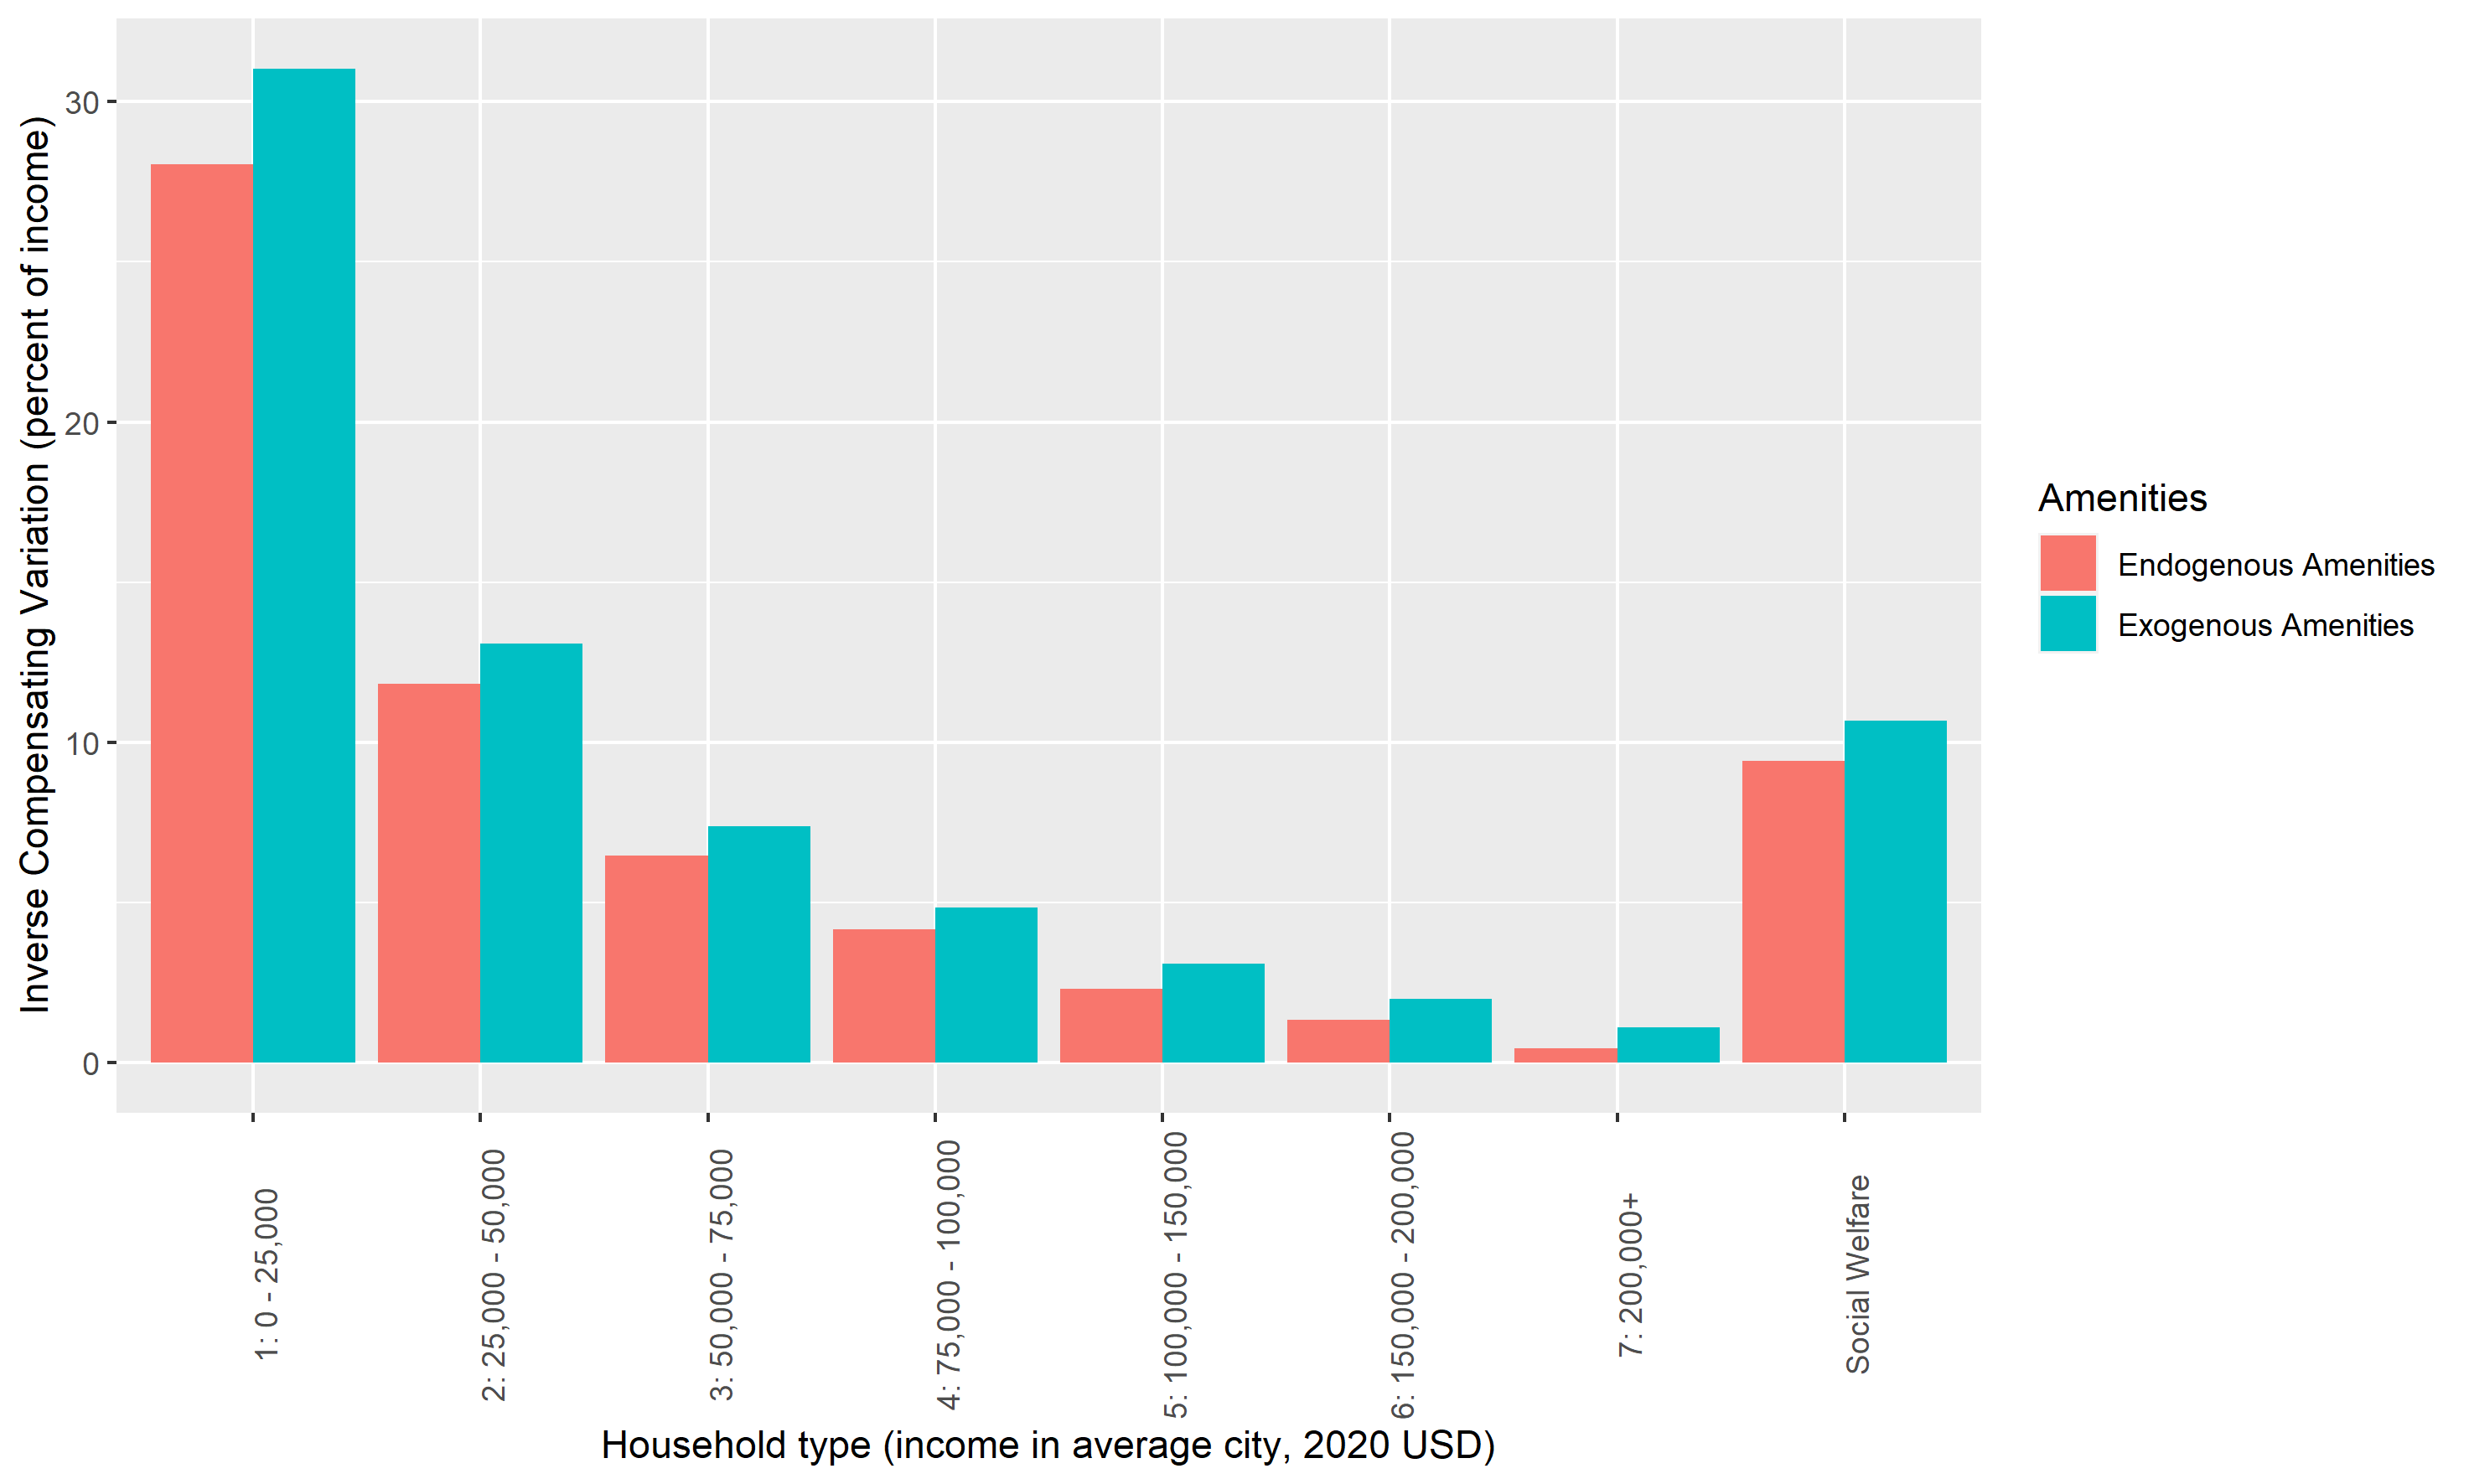
\includegraphics[width=1.1\textwidth]{Welfare.png}
	\end{center}
	\caption{Compensating variation by household type}\label{figure:welfare_ctfl}
\end{figure}

\paragraph*{} Figure \ref{figure:welfare_ctfl} shows that the social welfare of renters increases by a sizable $7.7\%$, and that this is primarily driven by the high share of households who make less than $\$50,000$ annually in a city with average productivity. Households who make less than $\$25,000$ gain the most, at $18\%$ of income, while those who make more than $\$200,000$ gain less than $y\%$. Welfare effects are similar by type when adopting an equivalent variation measure, albeit slightly attenuated. The results by income type are comparable to less ambitious reforms where there are no neighborhood choice externalities, e.g. \cite{Song} and \cite{kulka}. Moreover, the fact that all renters benefit in a presence of endogenous amenities challenges fiscal zoning exercises in the local public finance, e.g. \cite{calabresetal} and \cite{ineffTiebout}. These typically find aggregate welfare losses even when focusing only on households with no initial housing wealth. Finally, I find that landlords lose on average $8\%$ in land values after deregulation. This makes sense. In the theory, regulation makes housing consumption artificially large, and housing prices need to adjust upward to induce a supply response.

\paragraph*{Neighborhood choice externalities} 
How has the neighborhood choice externality affected the gains to deregulation we see in Figure \ref{figure:welfare_ctfl}? I propose two different methods to parse the welfare consequences of changing amenities $b(i, z)$ and neighborhood consumption values $V(i, z)$. 
\paragraph*{}
The first method asks what the benefits of deregulation would otherwise be if amenities were exogenous; amounting to repeating the counterfactual with $\Omega(z) = 0$ for every $z$. Another way of interpreting this is to say that all variation in amenity value by income type inferred from the data come from factors that are not caused by housing regulation. Figure \ref{figure:welfare_ctfl} reports the consequences of this counterfactual by income type in turquoise. The figure highlights two important things. First, the social welfare of renters is lower when amenities are endogenous compared to when they are not, but only by roughly 2\% for an average household comprising a relatively small portion of welfare gains. Note that all potential welfare gains from regulation for renters must come from endogenous amenities, as otherwise regulation can only distort housing consumption relative to the unregulated competitive equilibrium. The small differences in social welfare are in stark contrast to other papers studying zoning reforms quantitatively, namely \cite{calabresetal}. Second, the figure highlights the distributional effects of the endogenous amenities channel. The differences in welfare between the exogenous and endogenous models are roughly $-3\%$ for the lowest income type and $1\%$ for the highest income type, respectively. This is not surprising, as lower income households tend to decrease the amenities in locations for which they sort. This does not happen when amenities are held fixed.  

\paragraph*{THIS DECOMPOSITION IS A WORK IN PROGRESS. LET'S DISCUSS.}
The second method relies on decomposing welfare changes into amenity and consumption components. Consider the welfare measure $\boldsymbol{W}(z)$, defined in Equation \eqref{Welfare}. For some variable $x$, let $\hat{x}$ denote the ratio between its value at counterfactual and baseline. For example, $\hat{\boldsymbol{W}}(z)$ is the ratio between baseline and counterfactual welfare. As is well known, $\hat{\boldsymbol{W}}(z)$ can be expressed as follows

\begin{equation}\label{Welfare:Rep}
\hat{\boldsymbol{W}}(z) = \bigg[ \sum_{c \in \mathbb{C}} f(c, z) \big[\sum_{i \in N(c)}f_{c}(i, z)\hat{V_{e}}(i, z)^{\rho}\hat{b}(i, z)^{\rho}\big]^{\frac{\theta}{\rho}} \bigg]^{\frac{1}{\theta}}
\end{equation}
where $V_{e}(i, z) := e^{V(i, z)}$, $f(c, z)$ is the fraction of type $z$ agents in city $c$ at baseline, and $f_{c}(i, z)$ is the fraction of city $c$ households of type $z$ in neighborhood $i$ at baseline. This says that the change in aggregate welfare is some aggregation of changes in local welfare weighted by populations at baseline. Equation \eqref{Welfare:Rep} can be multiplicatively decomposed into three components


\begin{eqnarray*}\label{Welfare:Decomp}
	\hat{\boldsymbol{W}}(z) = & 	\bigg[ \sum_{c \in \mathbb{C}} f(c, z) \big[\sum_{i \in N(c)}f_{c}(i, z)\hat{b}(i, z)^{\rho}\big]^{\frac{\theta}{\rho}} \bigg]^{\frac{1}{\theta}} \times & \quad \text{(Amenity component)} \\
	& \bigg[ \sum_{c \in \mathbb{C}} f(c, z) \big[\sum_{i \in N(c)}f_{c}(i, z)\hat{V_{e}}(i, z)^{\rho}\big]^{\frac{\theta}{\rho}} \bigg]^{\frac{1}{\theta}} \times & \quad \text{(Consumption component)} \\
	& \xi(z) & \quad \text{(Residual)}
\end{eqnarray*}
$\xi(z)$ captures any effects induced by correlation between amenity and income growth across locations. 

\paragraph*{}
The first method points toward the idea that the neighborhood choice externality 1) matters relatively little when compared to housing affordability for the average household and 2) has important distributional consequences. These findings are best interpreted in the context of theory in Section \ref{Theory:Externality}. In this theory, I contrast two models; one where strong income sorting introduces the potential for minimum lot size regulation to benefit all renters, and one where relatively weak income sorting causes regulation to push lower income households to less desirable neighborhoods. The finding that distributional consequences matter suggests that the later model better characterizes the level of income sorting that we observe in the data. 

\paragraph*{Gentrification} Given distributional consequences associated with the externality, which neighborhoods benefit, and which neighborhoods lose? Taken together, Facts \ref{FIncomeDens} and \ref{Figure:StringencyStrong} suggest that high density neighborhoods benefit relative to low density neighborhoods within superstar cities. The model also makes this prediction. In Figure \ref{figure:gentrification}, I compare the income density gradient for both the observed and counterfactual equilibrium separately for the superstar and non-superstar samples. Each panel corresponds to a sample of cities. Within each panel, I plot flexible regressions of income (demeaned by MSA) on the baseline density ranking. Purple and yellow lines correspond to counterfactual and baseline income data, respectively. In Figure (xx) of Appendix (xx), I additionally reconstruct Figure \ref{Figure:IncomeSortingStrong} treating counterfactual incomes as data.

\begin{figure}[htbp!]
	
	\makebox[\textwidth]{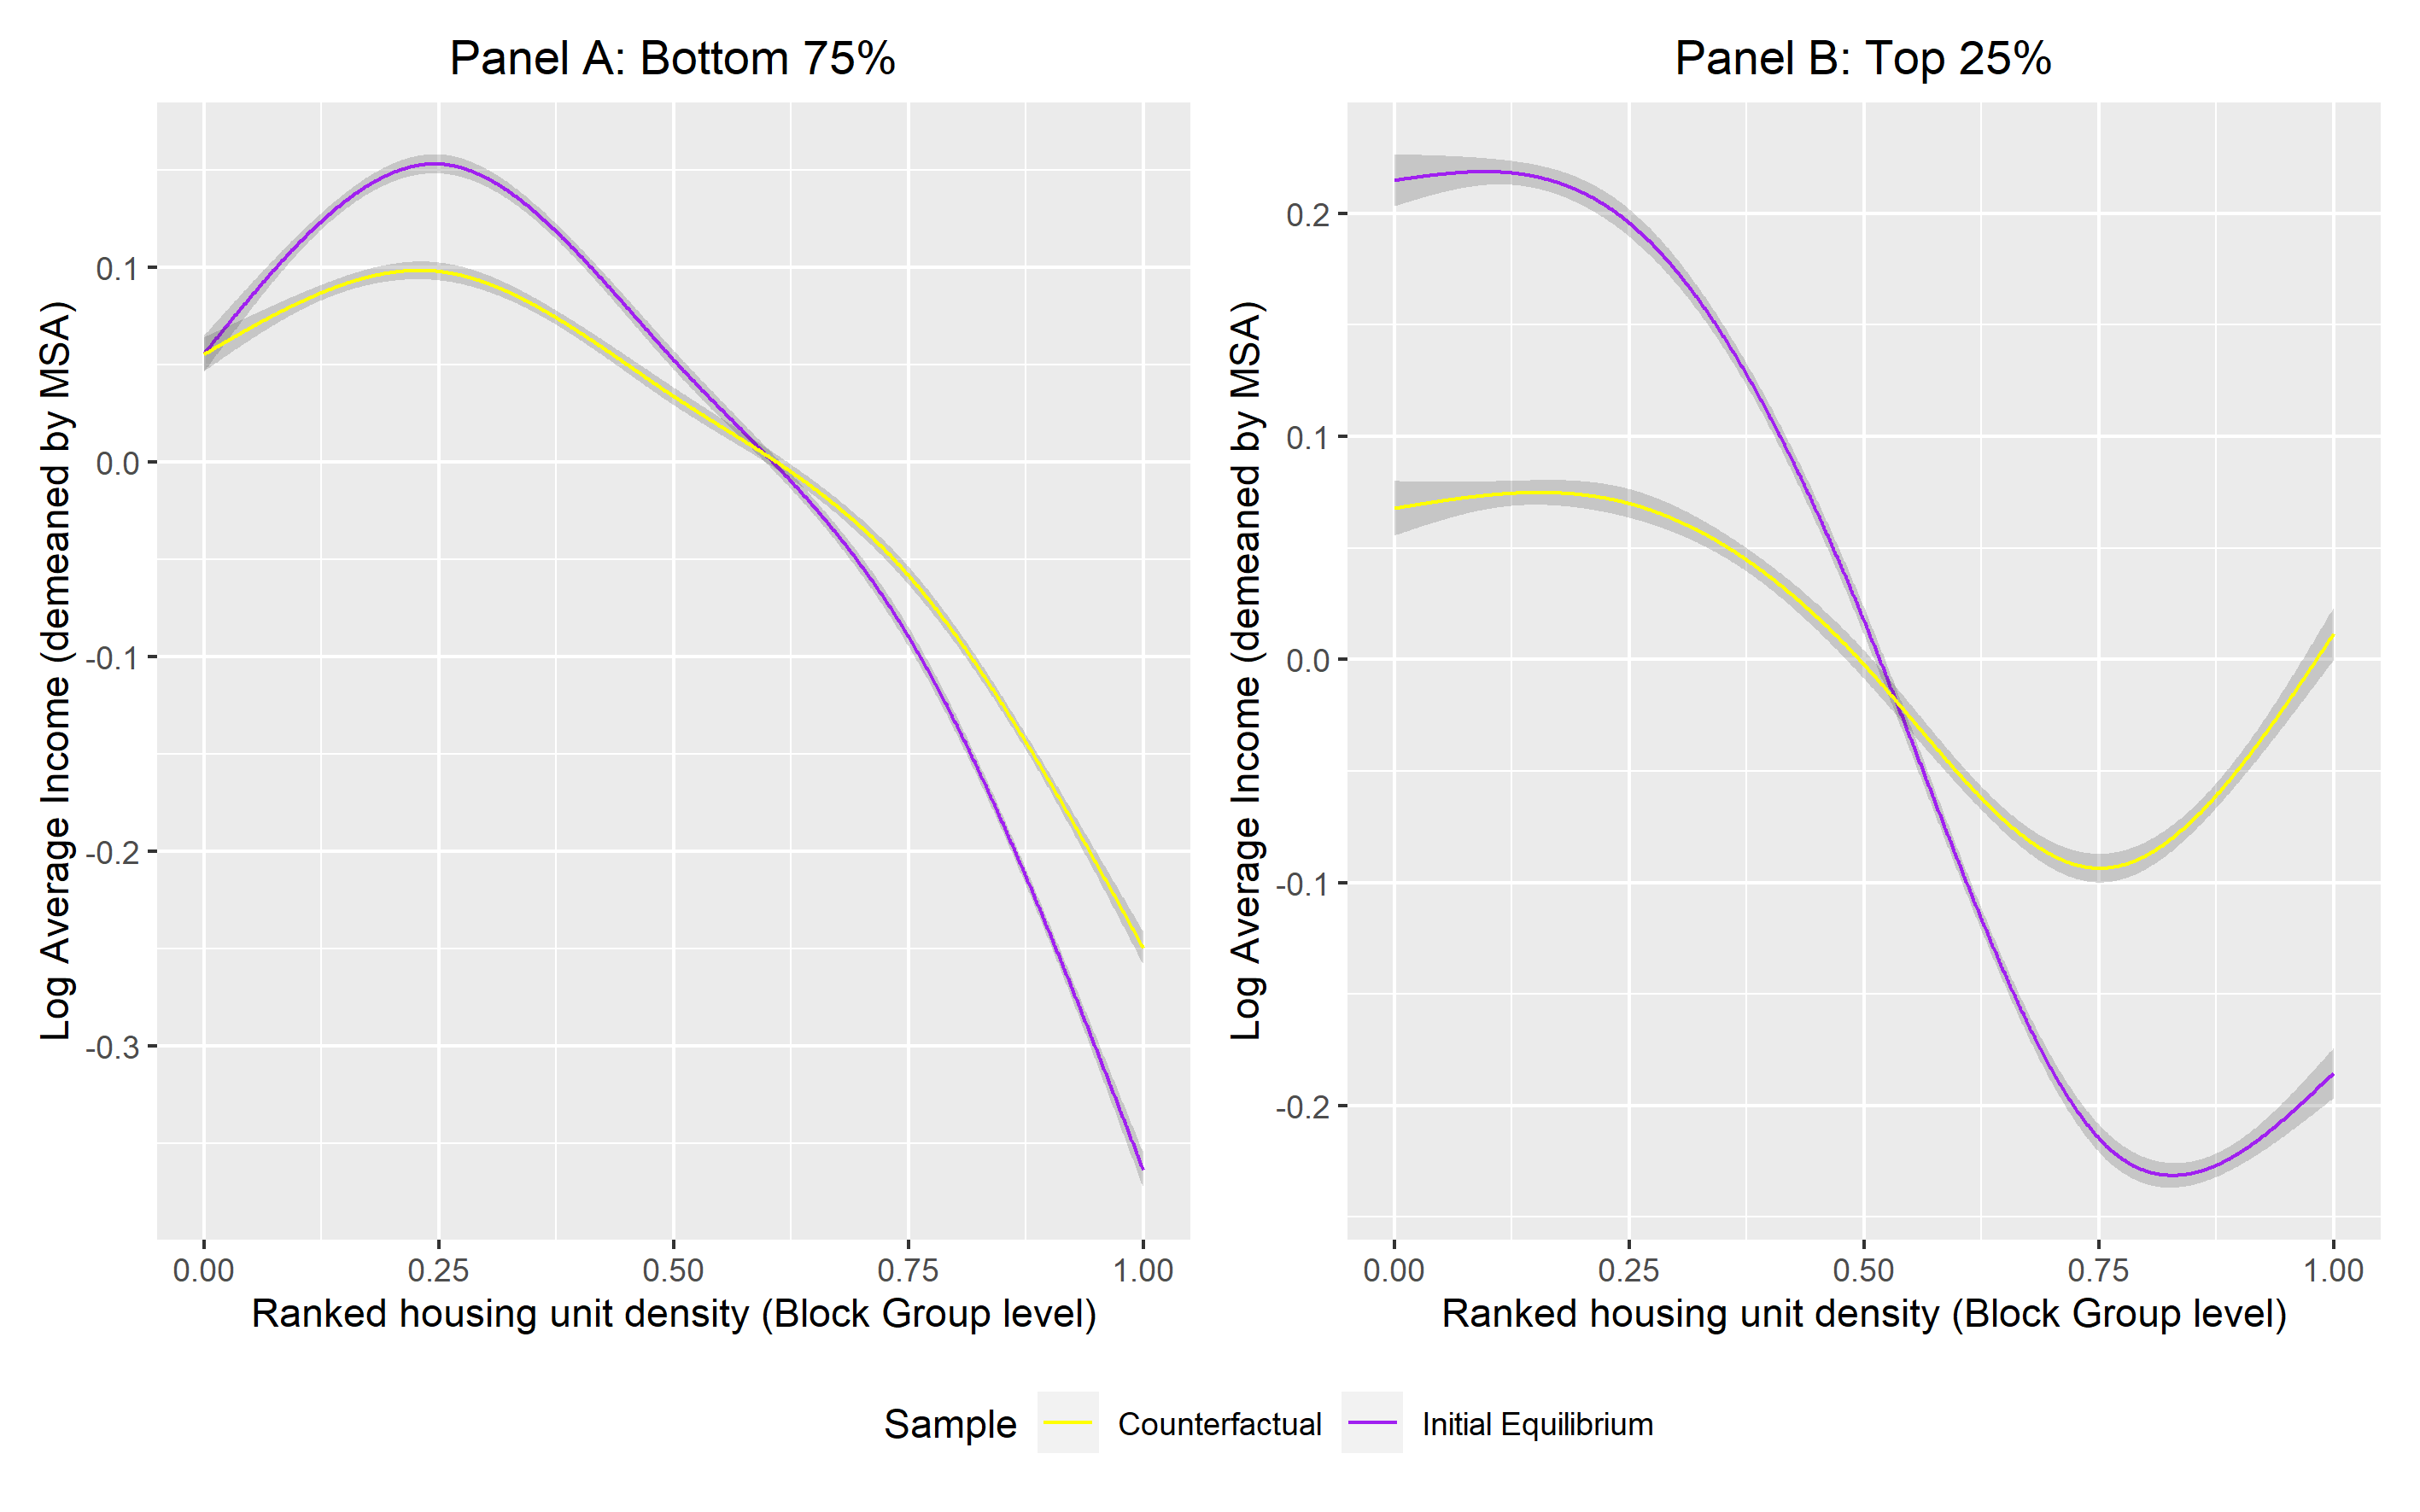
\includegraphics[width=\textwidth]{IncomeDensityGradCtfl.png}}
	
	\caption{Gentrification}\label{figure:gentrification}
	
\end{figure}

\paragraph*{}
Figure \ref{figure:gentrification} shows the stark prediction made by the model. The highest density neighborhoods in superstar cities observe a $23\%$ increase in their income relative to the city mean. Low density neighborhoods experience relatively less income declines spread out over more neighborhoods. On the other hand, cities in the non-superstar sample see little change to their income-density gradient, suggesting that minimum lot sizes tend to not be very binding in them or there is very little variation across space. To examine how much the income-density gradient has increased in superstar cities, I perform a linear regression of demeaned income on density in the superstar sample for both baseline and counterfactual data. I find that the differences in the income density gradient between superstars and non-superstars (Fact \ref{FIncomeDens}) disappears entirely in the counterfactual. This suggests that variation in regulation across space can account for \textit{all} differences in income sorting on density in expensive cities. In absolute terms, the average income density gradient in superstar cities increases from approximately $-0.65$ to $-0.37$ log points, a drop in magnitude of almost half. This is commensurate with the idea that income sorting in the absence of regulation is not strong, which puts a limit on the negative externalities associated with too many low income households crowding rich neighborhoods (Section \ref{Theory:Externality}). 

\paragraph*{Aggregate labour productivity} I find that complete deregulation increases aggregate labour productivity by only $0.45 \%$-- equivalent to roughly a fourth of a typical year of growth in the US. In contrast to the literature, \cite{durantonpugaurbgrowth} find that eliminating housing supply restrictions in superstar cities would increase output per person by around $8.2\%$. \cite{hseihmoretti} estimate the number to be $3.2\%$ in an exercise where they increase the housing supply elasticity in San Jose, San Francisco and New York. In the context of my model, the different findings can only be rationalized in two ways. On one hand, there may not be much movement across cities. On the other hand, this can be driven by the income sorting effect offsetting the influx of households into productive cities, considering lot sizes tend to be more stringent in them (see Fact \ref{FStringency}). To test both hypotheses, I plot the growth rate in the number of households against the growth rate in the average household income type $z$ across all cities in Figure \ref{figure:city_inc_sorting}, with each city representing a circle that is coloured by productivity and has a radius proportional to the city population. The figure very clearly rules out that there isn't much movement across cities. In general, we see a net inflow of households in cities with higher wages and housing prices. Table (xx) in Appendix (xx) shows high correlations between both counterfactual city household and income growth rates against observed housing prices, wages and the stringency measure $I(i)$ derived in the model and used the empirical work. 

\begin{figure}[htbp!]
	
	\makebox[\textwidth]{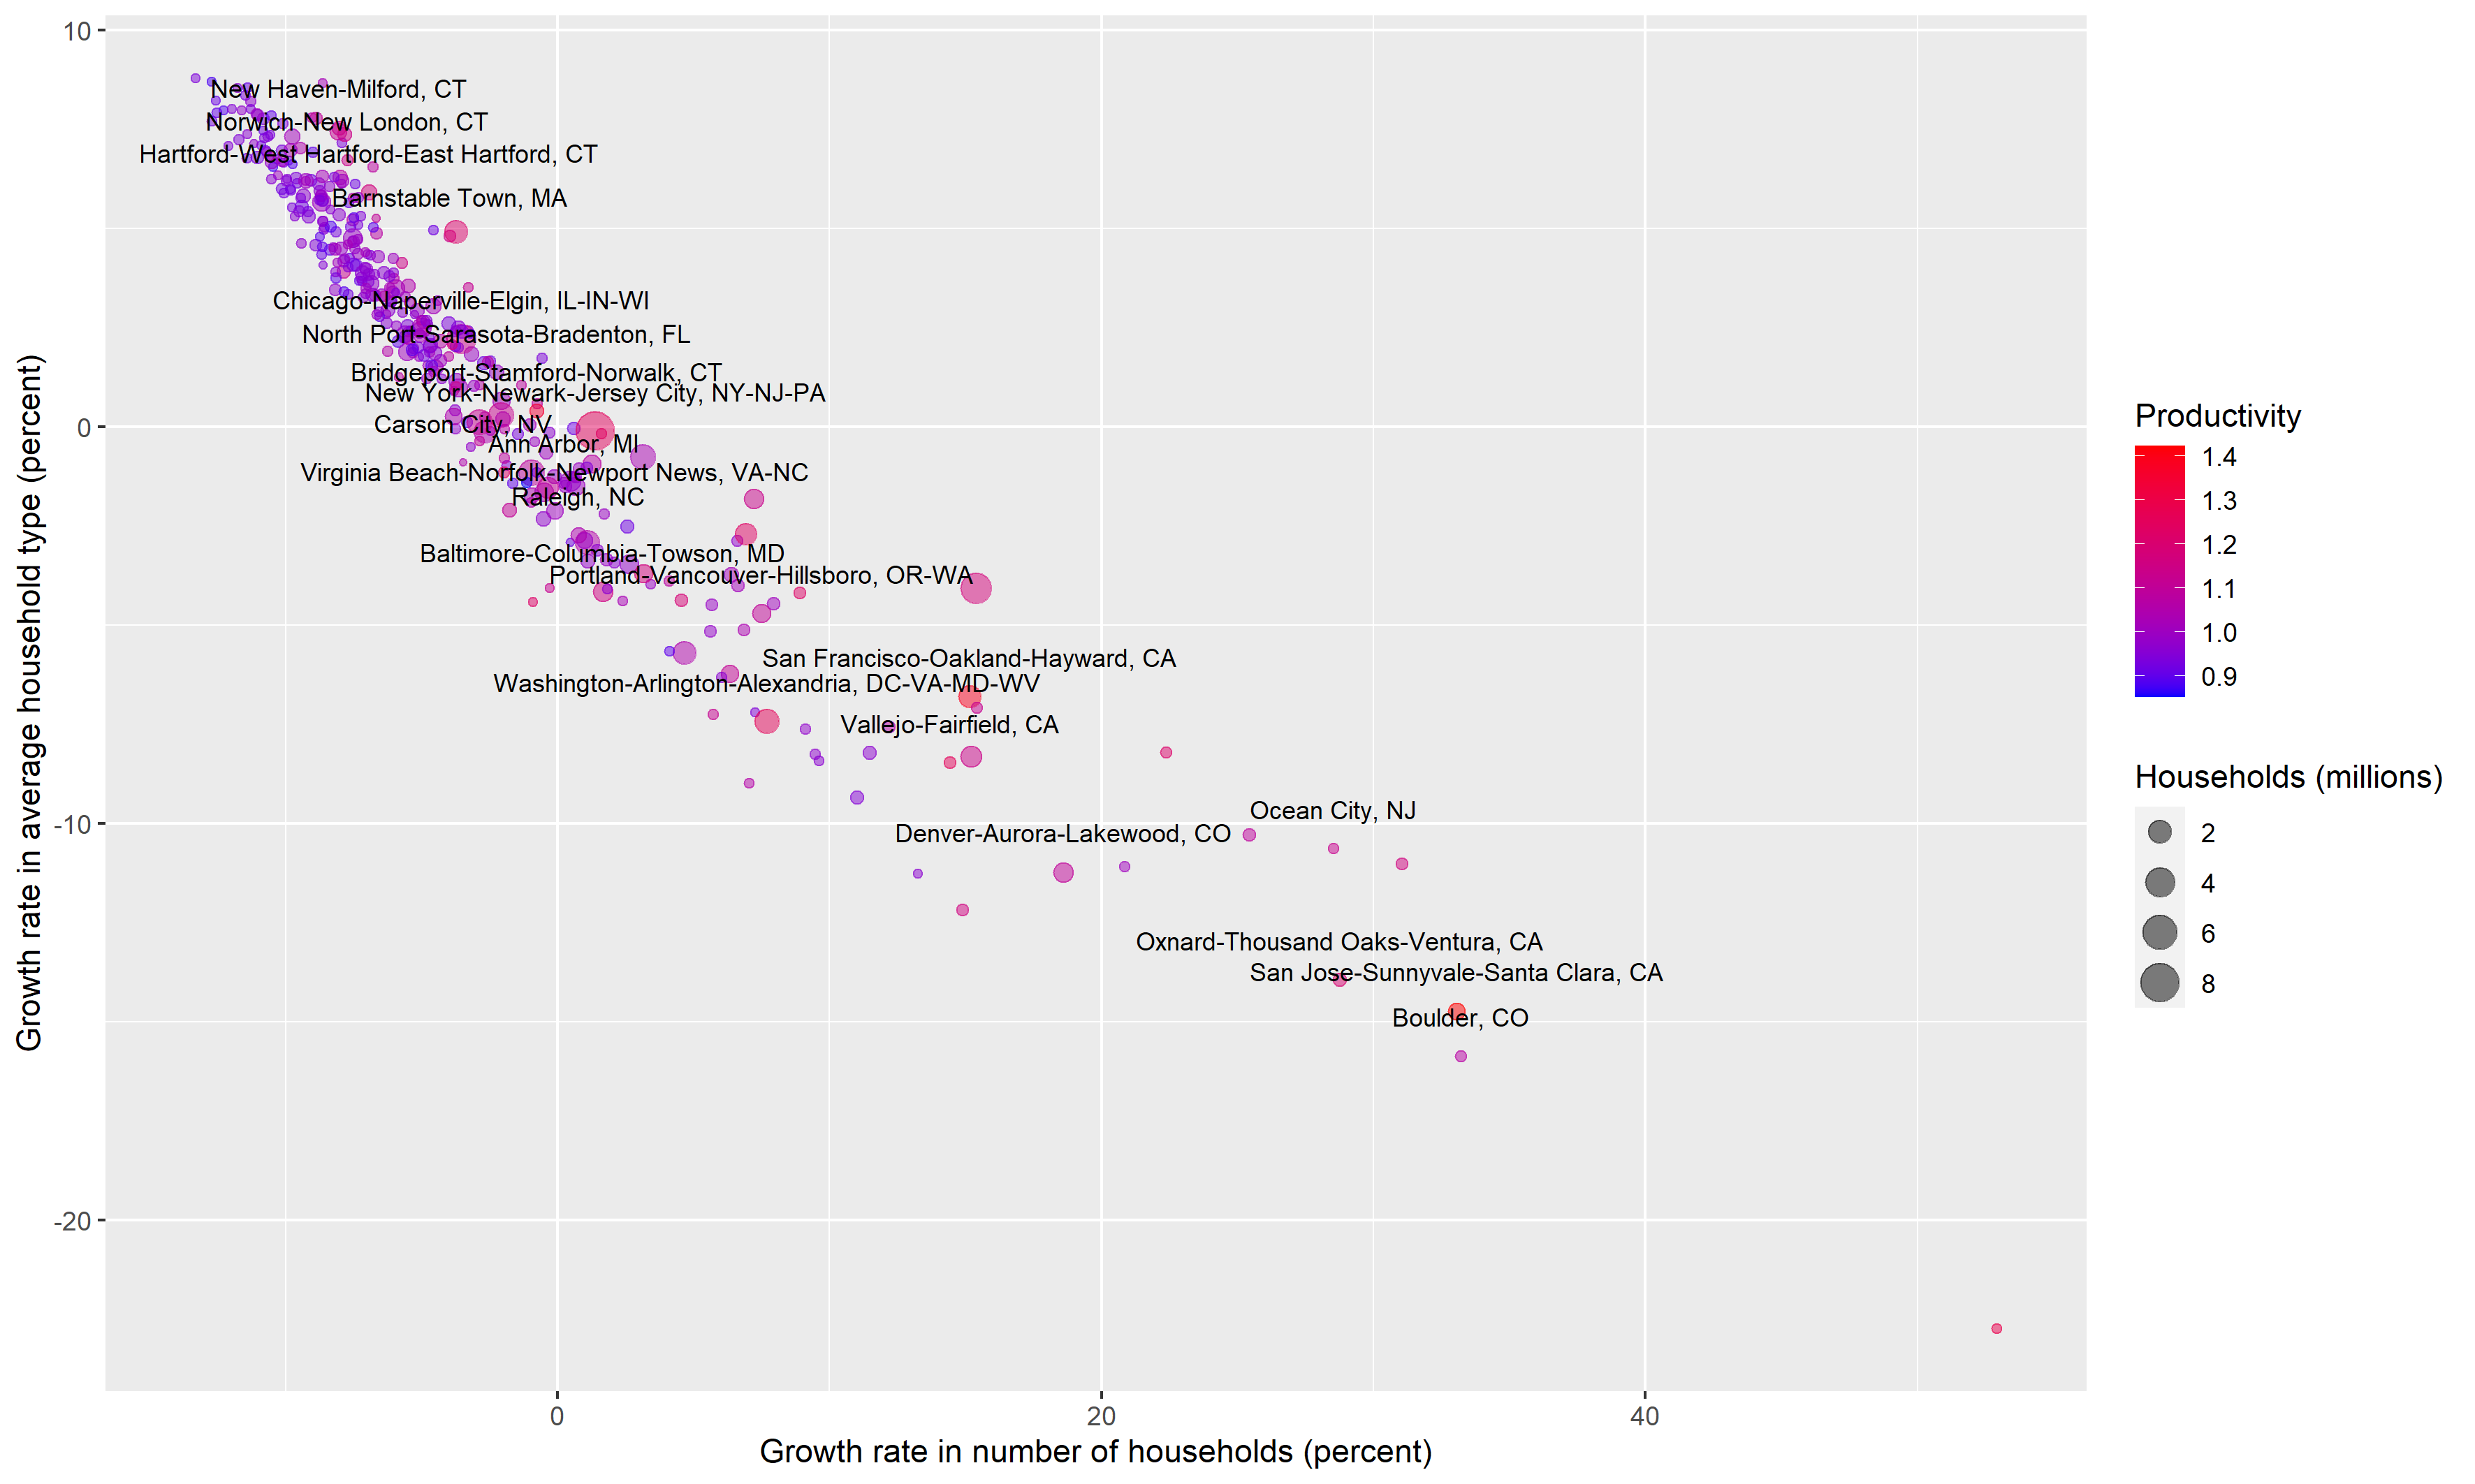
\includegraphics[width=\textwidth]{IncomeSortingMovement.png}}
	
	\caption{City Income Sorting. The $y$ axis is defined as the change in the average income that a household could earn in an average city. Correlation between the growth rate in the number of households productivity is approximately $50\%$, and this correlation is $60\%$ for unadjusted housing prices.  Cities on the top left (high income, negative population growth) tend to have low productivity, and cities with higher productivity tend to be in the bottom left.}\label{figure:city_inc_sorting}
	
\end{figure}

\paragraph*{}
To better quantify how income sorting has attenuated aggregate productivity growth in response to reform, I consider the following counterfactual exercise. I calculate what aggregate productivity would be if 1) cities had household growth as predicted by deregulation and 2) average income in each city remained at observed levels. This exercise yields an aggregate productivity of 1.55\%, which is three times higher than what is predicted when income sorting occurs.

\paragraph*{Landlords in regulated neighborhoods}
Given that all renters are better off, how can the model rationalize why minimum lot sizes are frequently imposed? I find that land values on average decrease by a larger amount in initially stringent neighborhoods. This is commensurate with the idea that homeowners impose land use restrictions to maximize their land values \citep{parkho, HILBER2013, homevoterhypothesis}. Theoretically, there are two competing effects that determine the relationship between land value growth and initial stringency. On one hand, stringent regulation distorts housing consumption and decreases neighborhood demand. On the other hand, neighborhood demand increases when stringent regulation increases neighborhood affluence. I find that, in an equilibrium where amenities are endogenous, land values are negatively related to initial levels of neighborhood stringency, but \textit{positively} related when amenities are exogenous. In Figure \ref{figure:landlords}, I plot log differences in land values against stringency for neighborhoods with initially positive stringency, along with linear estimates for the endogenous amenities counterfactual (red) and exogenous counterfactual (blue). 


\begin{figure}[htbp!]
	
	\makebox[\textwidth]{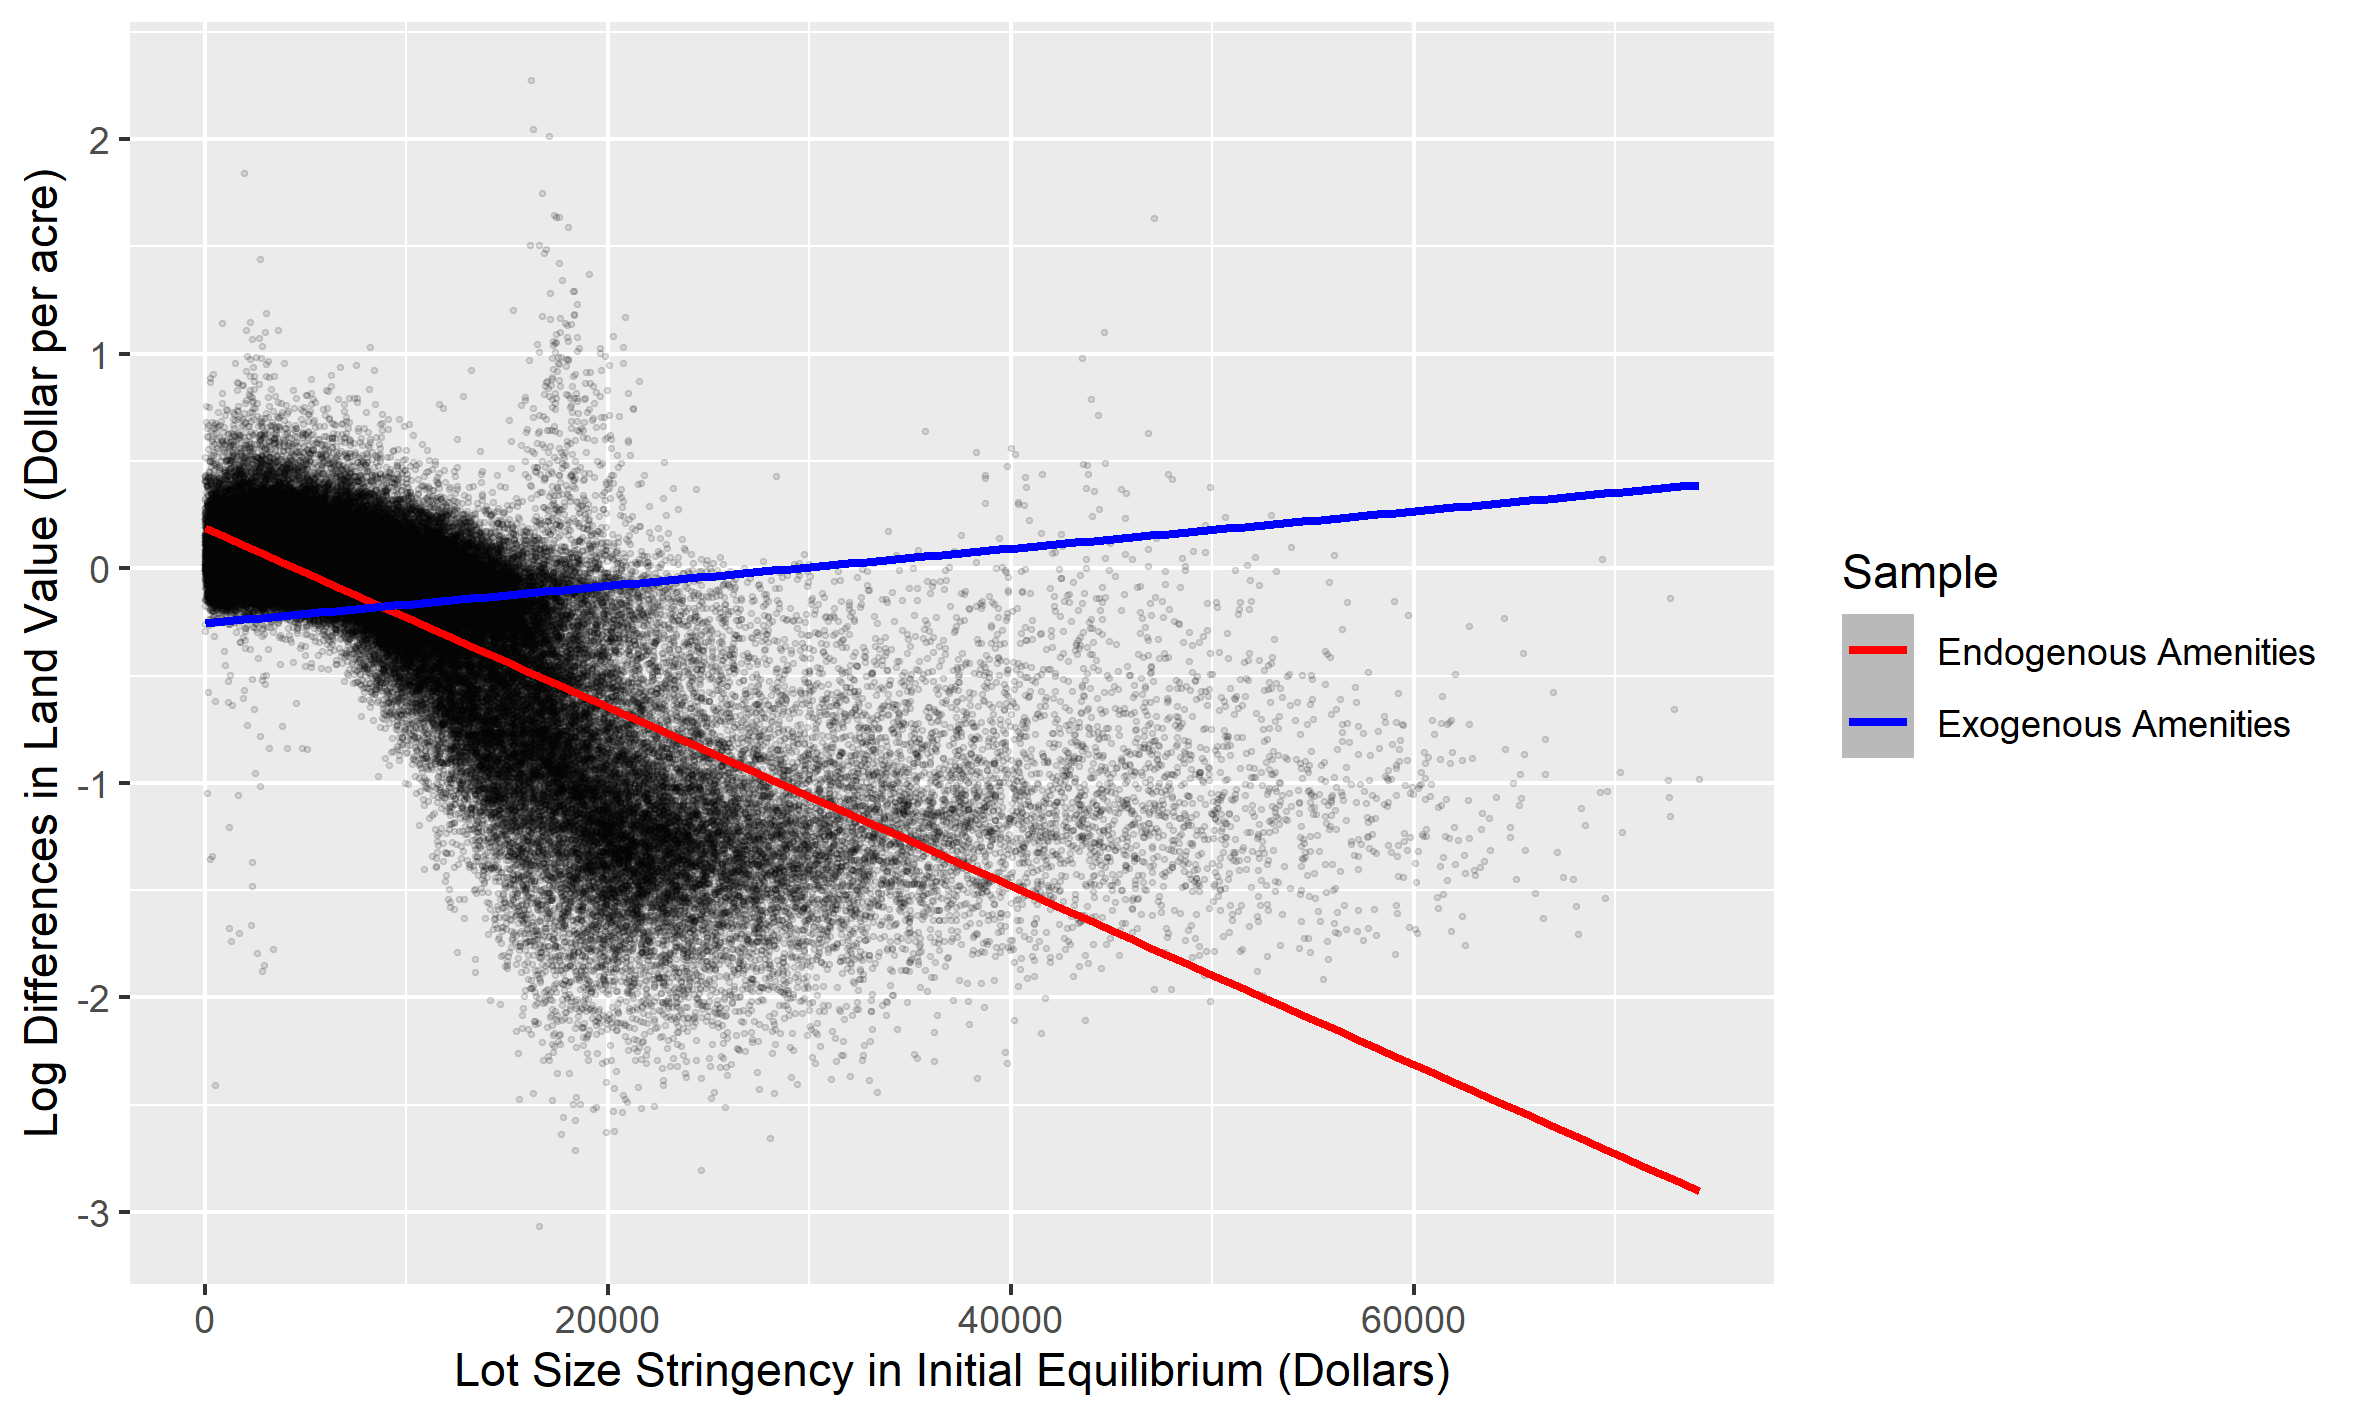
\includegraphics[width=\textwidth]{StringencyChangeLandVal.png}}
	
	\caption{Changes in land values by regulatory stringency in the baseline equilibrium.}\label{figure:landlords}
	
\end{figure}

\paragraph*{Robustness} Results all hold when considering a multitude of production technologies, including agglomeration economies at the household level, imperfect substitutes by education, and skill-biased agglomeration economies as estimated in \cite{diamond2016}, \cite{card}, and \cite{Combes_review}. For example, specifying that productivity responds to city population with an elasticity of $0.05$ changes aggregate productivity growth from $0.45$ to $0.7$. Differentiating income types by college and non-college educated workers whose substitution elasticity in production is $1.3$ \cite{card} changes productivity growth to $0.54$. Results are also robust to all confidence intervals and wildly different parameter choices for $\theta$, $\rho$, and $\Omega(z)$. Overall, I'm super confident with robustness, though I am less confident in other data cleaning areas were it is hard to test the model repeatedly to small changes in data cleaning procedures. Doing my best on this front. 

\subsection{Deregulation in superstar cities}
Have results, will write up soon. Theory suggests heterogenous affects of neighborhood choice that depend on housing expenditure share, housing supply elasticities, etc (I thank Nate for this suggestion). Also have results for incomplete deregulation that look more or less similar (attenuated slightly). 

\subsection{Socially optimal regulation}
Social planners problem + solution algorithm coming soon! What would optimal minimum lot sizes look like? If I find an interesting pattern that can be explained (i.e. keep high regulations in neighborhoods with relatively high fundamental amenities for the rich) then keep it in. Still a computational challenge since utility in the model is not everywhere differentiable. 


\section{Conclusion}

	\newpage\newpage
	\scriptsize
	\bibliography{references.bib}
	
	\newpage
	\appendix
	\normalsize
	\section{Appendix: Data and Facts Continued}\label{DataandFactsContinued}
	
	\subsection{Data Construction} \label{Appendix:DataConstruction}
	
	
	\subsection{Constructing Minimum Lot sizes} \label{Appendix:MinimumLotSizes}
	
	\subsection{Robustness of Facts to Alternative Specifications}\label{Appendix:Robustness}
	
	\paragraph*{Weights and sample definitions} Facts \ref{FIncomeDens} and \ref{FStringency} hold for multiple definitions of "superstar" cities. That is, for when superstar cities are defined to be in the top decile of density and housing prices, and for the top half and bottom half, respectively. The results also hold when assigning each city equal weight in the sample, rather than an unweighted regression across block groups. 
	
	\paragraph*{Across Time}  Strong differences in the income density gradient were even larger in the past. Using the 2008-2012 pooled ACS, the "single crossing property" in Panel B of Figure \ref{FIncomeDens} holds both conditional on and unconditional on controls. This suggests rapid gentrification happening in the high density neighborhoods of expensive cities, and is consistent with minimum lot sizes becoming slightly less stringent over time given the spatial variation in stringency within cities (Fact \ref{FStringency}). 
	
	\paragraph*{Distance to CBD}
	
	\paragraph*{Educational composition of neighborhoods}
	
	\paragraph*{Selection of controls}
	
	
	
	\newpage
	\section{Appendix: Theory}\label{TheoryAppendix}
	
	
	\subsection{Microfoundations for endogenous amenities channel}\label{microfoundations}
	
	\paragraph*{}
	
	In this section, I provide two approximate microfoundations for the relationship in Equation \eqref{endoamen}. These microfoundations correspond exactly to Equation \eqref{endoamen} in a given neighborhood whenever the mininum lot size in the regulated zone is zero (in other words, when a block group is assigned no minimum lot size regulation at all).  
	
	\paragraph*{Local Dixit-Stiglitz market with a disutility of density}
	
	
	
	\paragraph*{Local public goods financed through income taxes}
	
	
	\subsection{Proof of Proposition \ref{Prop:ReproduceFacts}}\label{Proof:ReproduceFacts}
	
	\paragraph*{}
	Proposition \ref{Prop:ReproduceFacts} has three parts. First, it says that city $c_{1}$ is relatively more affluent than $c_{0}$. Second, it says that the regulated neighborhood $i_{c1}$ is less dense than the associated unregulated neighborhood $i_{c0}$ in every city $c$. Third, city $c_{1}$ has a stronger income-density gradient. These three statements are true because of only differences in labour productivity across cities $c_{0}$ and $c_{1}$ and similar physical minimum lot sizes $\bar{l}$ in the regulated neighborhoods $i_{c1}$ in each city. These statements require that city $c_{1}$ is sufficiently more productive $\frac{\iota(c_{1})}{\iota(c_{0})} > k$ for some $k > 1$, and the physical minimum lot size $\bar{l}$ in the regulated neighborhoods $i_{c1}$ is sufficiently large to limit that density that would otherwise appear in equilibrium. All other parameters governing housing supply and demand in each neighborhood are purposefully identical. In what follows, note that we assume a perfect mobility equilibrium for this proof and thus a spatial equilibrium is a set of allocations across neighborhoods $L(i, z)$ such that $V(i, z) \leq V(z)$ for some $V(z)$ and all neighborhoods in each city $i$ such that $V(i, z) < V(z) \implies L(i, z) = 0$. Also note that preferences are Cobb-Douglas, $\bar{A} = 0$. Lastly, recall that we make no distinction between regulated and unregulated zones to make the exposition as simple as necessary. 
	
	\paragraph*{}Before proving each statement separately, I start with a few lemmas that will be used:
	
	\begin{enumerate}
		\item	If $\frac{\iota(c_{1})}{\iota(c_{0})} > 1$, then $P(i_{c_{1}1}) > P(i_{c_{0}1})$ and  $P(i_{c_{1}0}) > P(i_{c_{0}0})$ in spatial equilibrium. That is, regulated neighborhoods command a higher price per unit of housing services in the more productive city, and the same is true for unregulated neighborhoods. 
		
		Proof: $P(i_{c_{1}0}) \leq P(i_{c_{0}0})$ implies $V(i_{c_{1}0}, z) > V(i_{c_{0}0}, z)$ for all income types $z$ since utility is strictly decreasing in prices and strictly increasing in productivity $\iota(c)$. This means that no households of any income types will sort into $i_{c_{1}0}$. In spatial equilibrium, zero population implies zero housing prices under market clearing, which is not consistent with finite utility; a contradiction. The same argument applies for regulated neighborhoods $i_{c1}$ because they are assumed to have the exact same physical minimum lot size $\bar{l}$ in each city and utility is strictly decreasing in prices per unit of housing services.
		
		\item Let $L(z)$ be the exogenous mass of type $z$ households. If $\bar{l} > \frac{1}{4}L(z_{0}) + \frac{1}{4}L(z_{1})$, then the regulated neighborhood in city $c_{1}$ $i_{c_{1}1}$ has a binding minimum lot size for at least the lowest income type $z_{0}$.
		
		Proof: Suppose minimum lot sizes in $i_{c_{1}1}$ were not binding for any income type. Since neighborhoods within each city are identical on every dimension but for regulation, it must be that city $c_{1}$ has a symmetric equilibrium across each of its neighborhoods. That is, $L(i_{c_{1}1}) = L(i_{c_{1}0}) = \frac{1}{2}L(c_{1})$, where $L$ is the total population of households in a neighborhood or city. However, by Lemma 1, each neighborhood in $c_{1}$ must command higher prices per unit of housing services than their corresponding neighborhoods in $c_{0}$ which requires a higher total population in $c_{1}$. This means that $L(c_{1}) > L(c_{0})$ and so $L(c_{1}) > \frac{1}{2}L(z_{0}) + \frac{1}{2}L(z_{1})$ which implies $L(i_{c_{1}0}) > \frac{1}{4}L(z_{0}) + \frac{1}{4}L(z_{1})$. Since each neighborhood has unit land mass, there cannot be more households than the minimum lot size. Hence, $L(i_{c_{1}0}) \leq \bar{l} < \frac{1}{4}L(z_{0}) + \frac{1}{4}L(z_{1})$. This is a contradiction.
		
		\item There exists a $k$ such that $\frac{\iota(c_{1})}{\iota(c_{0})} > k$ implies that the minimum lot size in the non-superstar city $c_{0}$ is not binding. 
		
		Proof: As $\frac{\iota(c_{1})}{\iota(c_{0})} \to \infty$ holding $\iota(c_{0})$ fixed, it must be that $P(i_{c_{0}1})$ and $P(i_{c_{0}0})$ become arbitrarily small to ensure spatial equilibrium, see Equation \eqref{utility}. For prices arbitrarily small, the value of a minimum lot $\bar{l}P^{1 + \epsilon}$ for prices $P$ will always be non-binding below desired spending on housing services by the lowest income type $\beta \iota(c_{0}) z_{0}$. 
		
	\end{enumerate}
	With each lemma, I prove each statement separately assuming $\frac{\iota(c_{1})}{\iota(c_{0})} > k > 1$ for some $k$ that is shown to exist, as well as $\bar{l} > \frac{1}{4}L(z_{0}) + \frac{1}{4}L(z_{1})$.
	
	\paragraph*{Statement 1} (City $c_{1}$ is more affluent) Since $V(i, z)$ is supermodular in regulation $l(i)$ and income $z$ (Equation \ref{supermodularity}), it must be the case that the $c_{1}$ regulated neighborhood is relatively more affluent $$L(i_{c_{1}1}, z_{1})/L(i_{c_{1}1}, z_{0}) > L(i_{c_{0}1}, z_{1})/L(i_{c_{0}1}, z_{0})$$ (note that the left hand side can take values of $\infty$ due to perfect income sorting). Moreover, the unregulated neighborhoods in both cities have the same level of affluence because $V(i, z)$ is equalized for both income types simultaneously because prices  must satisfy $\frac{P(i_{c_{1}1})}{P(i_{c_{0}1})} = \bigg[\frac{\iota(c_{1})}{\iota(c_{0})}\bigg]^{\frac{1}{\beta}}$ in spatial equilibrium. Since one neighborhood is strictly more affluent and all neighborhoods are as affluent in city $c_{1}$, this city is more affluent as a whole $$L(c_{1}, z_{1})/L(c_{1}, z_{0}) > L(c_{0}, z_{1})/L(c_{0}, z_{0})$$
	 
	
	\paragraph*{Statement 2} (Neighborhood $i_{c1}$ has weakly lower density of housing units relative to $i_{c0}$ with a strict inequality in $c_{1}$) Since minimum lot sizes under the above assumptions are not binding in $c_{0}$ and each neighborhood is identical within a city, each neighborhood in $c_{0}$ has the same density of households. Moreover, $i_{c_{1}1}$ must have a strictly lower price per unit of housing services relative to $i_{c_{1}0}$ in $c_{1}$ to compensate for the overconsumption of housing services induced by binding regulation\footnote{Again, there are no differences in amenity value across neighborhoods. Each neighborhood is purposefully identical.}. A lower housing price is only commensurate with a lower total population of households because this neighborhood has relatively higher income than all other neighborhoods (else, total spending on housing services, and thus prices per unit of housing services, would be greater). Hence $i_{c_{1}1}$ has a lower population than $i_{c_{1}0}$, which means lower density since all neighborhoods have the same land mass.
	
	
	\paragraph*{Statement 3} ($c_{1}$ exhibits a larger income-density gradient than $c_{0}$) This follows directly from the fact that the minimum lot size is binding in $c_{1}$ and not in $c_{0}$, which causes income sorting as shown in the proof of  Statement 1. 
	
	\subsection{Proof of Proposition \ref{Prop:NeighborhoodChoiceExt}}\label{Proof:NeighborhoodChoiceExt}
	\paragraph*{}
	Proposition \ref{Prop:NeighborhoodChoiceExt} has two parts. The first is to show that the unregulated equilibrium (an equilibrium such that all minimum lot sizes are \textit{not} binding) is unique. Second, it says that imposing a marginal increase in a minimum lot size from this unregulated equilibrium in the rich neighborhood $i_{1}$ such that it is binding for type $z_{m}$ causes a Pareto improvement for all renters if a specific set of parametric assumptions hold. For what follows, we define utility derived from neighborhood $i$ for type $z$ as $\tilde{V}(i, z) := e^{V(i, z)}b(i, z)$ and note that we assume a perfect mobility equilibrium (that is, in the limit where the migration elasticities $\theta$ and $\rho$ are infinite). This means that a spatial equilibrium is defined as a set of allocations $L(i, z)$ such that $\tilde{V}(i, z) \leq \tilde{V}(z)$ for some $\tilde{V}(z)$ and all $i$ such that $\tilde{V}(i, z) < \tilde{V}(z) \implies L(i, z) = 0$. 
	
	\paragraph*{Uniqueness}
	I start by proving the first part. It is sufficient to show that the equilibrium is unique when setting minimum lot sizes to zero, or $l(i) = 0$ for every $i$. This is because any equilibrium where a positive minimum lot size is nonbinding in the consumption problem must look the same as if there were no minimum lot sizes at all-- see Equation \eqref{utility}. The idea is to show that there is a unique allocation of middle income types $L(i, z_{m})$ that satisfy the definition of a spatial equilibrium. Note that, by the assumed structure of fundamental amenities $\nu(i, z)$, we know that $L(i_{0}, z_{h}) = 0$ and $L(i_{1}, z_{l}) = 0$ in any equilibrium under any set of parameter values, so we need not be concerned about their location choices to show uniqueness. 
	
	\paragraph*{}
	Suppose, to arrive at a contradiction, that there are two or more distinct allocations of $z_{m}$ types that satisfy the spatial equilibrium condition. Pick any two distinct allocations and order them by the number of middle type households who in the rich neighborhood $i_{1}$,  $L_{0}(i_{1}, z_{m}) < L_{1}(i_{1}, z_{m})$.  Neighborhood $i_{1}$ in the maximal allocation $1$ must have the lowest average income of all other $i_{1}$ neighborhoods in the other equilibrium allocations\footnote{Since middle income types have the lowest income of any other type in the rich neighborhood, since we assumed that no low income types $z_{l}$ sort into $i_{1}$.}. Moreover, it must have the highest price per unit of housing services $P(i_{1})$ relative to other $i_{1}$ allocations because of the higher $z_{m}$ population and equal populations of $z_{h}$ types. The opposite must be true for neighborhood $i_{0}$ in the 1-allocation. Let $v_{0}$ be the utility level achieved by $z_{m}$ types in the $0$-allocation. Since prices are higher and incomes are lower in $i_{1}$ in the 1-allocation and the opposite is true in the 0-allocation, it must be that $$V_{1}(i_{0}, z_{m}) > v_{0} > V_{1}(i_{1}, z_{m})$$ which contradicts the fact that the 1-allocation must have $L_{1}(i_{1}, z_{m}) > 0$ and be a spatial equilibrium. Therefore, the existence of two or more distinct equilibria is not true.
	
	\paragraph*{Pareto improvements} I move to the second part of the proof. Consider a marginal change in the minimum lot size $l$ in $i_{1}$ around the unique unregulated equilibrium that causes regulation to be binding for $z_{m}$ types who may choose to live there, but not for $z_{h}$ types\footnote{This marginal change is possible because high income types $z_{h}$ have strictly higher income.}. I show that this marginal change induces population flows that are Pareto improving for all renters if and only if $k \Omega > \frac{\beta}{1 + \epsilon}$ for some $k > 0$ that may depend on endogenous objects in the unique unregulated equilibrium.
	
	\paragraph*{}
	 Consider such a marginal change in the minimum lot size $\partial l$ which must induce population flows of middle income types toward the poorer $i_{0}$ neighborhood, $\partial L(i_{0}, z_{m}) > 0$\footnote{This reallocation must happen because we assumed that $L(i, z_{m}) > 0$ in each neighborhood $i$ and so each neighborhood must offer equal utility levels for $z_{m}$ types in the unregulated equilibrium.}. The effect of this reallocation on utility offered in neighborhood $i_{0}$ for an arbitrary income type $z$ satisfies $$\partial \tilde{V}(i_{0}, z) = \tilde{V}(i_{0}, z)\bigg(V(i, z)\beta \partial \log P(i_{0}) + \Omega \partial \log I(i_{0}) \bigg)
	 $$
	where $I(i)$ is defined as the average income in neighborhood $i$. This holds because we assume preferences are Cobb-Douglas, or $\bar{A} = 0$ in Equation \eqref{utility}. We can decompose the expression above. Housing prices in equilibrium are isoelastic in total spending on housing (this can be derived easily by manipulating the housing market clearing condition noting that neighborhood $i_{0}$ is unregulated). This means that 
	$$\partial \log P(i_{0}) = \frac{1}{1 + \epsilon}\partial \log Y(i_{0})$$
	where $Y(i)$ is total income in $i$, $\sum_{z}zL(i, z)$. Moreover, the expression for $\partial \log Y(i)$ satisfies $\partial \log I(i) = \partial \log Y(i) - \partial \log L(i)$ where $L(i)$ is total population $L(i) = \sum_{z}L(i, z)$. Combining these expressions gets us $$\partial \tilde{V}(i_{0}, z) = \tilde{V}(i_{0}, z)\bigg( (\Omega - V(i, z)\frac{\beta}{1 + \epsilon}) \partial \log Y(i_{0}) - \Omega \partial \log L(i_{0})  \bigg)
	$$
	\paragraph*{}
	We can break down this expression even further. We know that $\partial \log L(i_{0}) = \frac{\partial L(i_{0}, z_{m})}{L(i_{0})}$ and $\partial \log Y(i_{0}) = \frac{z_{m}\partial L(i_{0}, z_{m})}{Y(i_{0})}$ and can substitute this into the equation above. So, to show that $\partial \tilde{V}(i_{0}, z) > 0$ it suffices to show that $\tilde{V}(i, z) \geq 0$ and $$(\Omega - V(i, z)\frac{\beta}{1 + \epsilon}) z_{m}L(i_{0}) - \Omega Y(i_{0}) \geq 0$$ 
	which is true if and only if $$k(z)\Omega \geq \frac{\beta}{1 + \epsilon}$$ where $k(z) := V(i, z)^{-1}(1 - \frac{Y(i_{0})}{z_{m}L(i_{0})})$. Note that $k(z) > 0$ for all $z$ since $Y(i_{0}) < z_{m}L(i_{0})$ at the initial unregulated equilibrium. Define $k := \max_{z}k(z)$. 
	
	\paragraph*{}
	I will use the derivation above as a lemma to complete the proof. If  $k\Omega \geq \frac{\beta}{1 + \epsilon}$ for the $k$ defined above, then reallocations of the middle income types to $i_{0}$ in transition to the new spatial equilibrium increase $\tilde{V}(i, z)$ for both types $z_{l}$ and $z_{m}$ agents who live in $i_{0}$. This is because $L(i_{0}, z) > 0$ in the new regulated equilibrium for $z \in \{z_{l}, z_{m}\}$, and so it must be the case that $\tilde{V}(i_{0}, z) = \max_{i}\tilde{V}(i, z)$ for each $z \in \{z_{l}, z_{m}\}$. Finally, we know that $\tilde{V}(i_{1}, z_{h})$ increases in transition to the new equilibrium because rents fall, average residential income increases and regulation is not binding for high types in $i_{1}$. Hence, we have that a marginal change in minimum lot sizes $\partial l$ induces changes in utility such that $$\partial \max_{i}\tilde{V}(i, z) \geq 0$$ for every income type $z$. Moreover, $\partial \max_{i}\tilde{V}(i, z_{h}) > 0$. This is the definition of a Pareto improvement (for renters only). 
	
	
	\subsection{Proof of Proposition \ref{Prop:NeighborhoodChoiceExt2}}\label{Proof:NeighborhoodChoiceExt2}
	
	\newpage
	
	
	\section{Appendix: Calibration}\label{Appendix:Calibration}
	
	\newpage
	
	\section{Appendix: Estimating $\Omega(z)$}\label{Appendix:Estimation}
	
	\subsection{Supplementary Estimation Tables} \label{Appendix:SupplementEstTables}
	\begin{table}[htbp]
		
\begin{tabular}{lccc} \hline
 & (1) & (2) & (3) \\
VARIABLES & ln Amenity (Low) & ln Amenity (Med) & ln Amenity (High) \\ \hline
\vspace{4pt} & \begin{footnotesize}\end{footnotesize} & \begin{footnotesize}\end{footnotesize} & \begin{footnotesize}\end{footnotesize} \\
ln Income & -0.0458*** & 0.0499*** & 0.1628*** \\
\vspace{4pt} & \begin{footnotesize}(0.0033)\end{footnotesize} & \begin{footnotesize}(0.0046)\end{footnotesize} & \begin{footnotesize}(0.0048)\end{footnotesize} \\
Slope Control & 0.0033*** & 0.0041*** & 0.0025*** \\
\vspace{4pt} & \begin{footnotesize}(0.0012)\end{footnotesize} & \begin{footnotesize}(0.0013)\end{footnotesize} & \begin{footnotesize}(0.0008)\end{footnotesize} \\
Local Slope Control & 0.0013*** & 0.0011** & -0.0005 \\
\vspace{4pt} & \begin{footnotesize}(0.0004)\end{footnotesize} & \begin{footnotesize}(0.0004)\end{footnotesize} & \begin{footnotesize}(0.0006)\end{footnotesize} \\
Outer Slope Control & -0.0004 & -0.0033 & -0.0009 \\
 & \begin{footnotesize}(0.0028)\end{footnotesize} & \begin{footnotesize}(0.0031)\end{footnotesize} & \begin{footnotesize}(0.0034)\end{footnotesize} \\
\vspace{4pt} & \begin{footnotesize}\end{footnotesize} & \begin{footnotesize}\end{footnotesize} & \begin{footnotesize}\end{footnotesize} \\
Observations & 170,951 & 171,045 & 165,317 \\
Specification & OLS & OLS & OLS \\
Donut & 0.75-1.25km & 0.75-1.25km & 0.75-1.25km \\
Base Controls & Yes & Yes & Yes \\
Amen/Topo Controls & No & No & No \\
 Density Control & No & No & No \\ \hline
\multicolumn{4}{c}{\begin{footnotesize} Robust standard errors in parentheses\end{footnotesize}} \\
\multicolumn{4}{c}{\begin{footnotesize} *** p$<$0.01, ** p$<$0.05, * p$<$0.1\end{footnotesize}} \\
\end{tabular}


		\caption{Baseline OLS Specifications by income group. Columns are ordered by income group. "Donut Slope Control" is the average slope within the block group plus a buffer with length equal to $d_{1}$. "Local Slope Control" is the average slope within the block group. "Base Controls" include travel time, building age, public transport and bus shares in commuting and CBD distance. "Amen/Topo" controls include various amenities (density of coffee shops, parks, restaurants) and various topographic features (cover of different types of forest such as deciduous or evergreen, wetlands, perennial snow cover). "Density Control" is the within-MSA density ranking of the block group.}\label{table:OLS}
	\end{table}
	
	\begin{table}[htbp]
		
\begin{tabular}{lccccc} \hline
 & (1) & (2) & (3) & (4) & (5) \\
VARIABLES & ln Amenity & ln Amenity & ln Amenity & ln Amenity & ln Amenity \\ \hline
\vspace{4pt} & \begin{footnotesize}\end{footnotesize} & \begin{footnotesize}\end{footnotesize} & \begin{footnotesize}\end{footnotesize} & \begin{footnotesize}\end{footnotesize} & \begin{footnotesize}\end{footnotesize} \\
ln Income & 0.0550*** & 0.1990*** & 0.2243*** & 0.2414*** & 0.3242*** \\
\vspace{4pt} & \begin{footnotesize}(0.0029)\end{footnotesize} & \begin{footnotesize}(0.0300)\end{footnotesize} & \begin{footnotesize}(0.0318)\end{footnotesize} & \begin{footnotesize}(0.0318)\end{footnotesize} & \begin{footnotesize}(0.0415)\end{footnotesize} \\
Slope Control & 0.0030*** & -0.0014* & -0.0018** & -0.0016** & -0.0041*** \\
\vspace{4pt} & \begin{footnotesize}(0.0010)\end{footnotesize} & \begin{footnotesize}(0.0008)\end{footnotesize} & \begin{footnotesize}(0.0008)\end{footnotesize} & \begin{footnotesize}(0.0008)\end{footnotesize} & \begin{footnotesize}(0.0010)\end{footnotesize} \\
Local Slope Control & 0.0016*** & 0.0005 & -0.0008 & -0.0012* & -0.0015* \\
\vspace{4pt} & \begin{footnotesize}(0.0005)\end{footnotesize} & \begin{footnotesize}(0.0006)\end{footnotesize} & \begin{footnotesize}(0.0006)\end{footnotesize} & \begin{footnotesize}(0.0007)\end{footnotesize} & \begin{footnotesize}(0.0008)\end{footnotesize} \\
Outer Slope Control & -0.0052 & 0.0009 & 0.0050 & 0.0053* & 0.0063* \\
 & \begin{footnotesize}(0.0038)\end{footnotesize} & \begin{footnotesize}(0.0039)\end{footnotesize} & \begin{footnotesize}(0.0033)\end{footnotesize} & \begin{footnotesize}(0.0031)\end{footnotesize} & \begin{footnotesize}(0.0036)\end{footnotesize} \\
\vspace{4pt} & \begin{footnotesize}\end{footnotesize} & \begin{footnotesize}\end{footnotesize} & \begin{footnotesize}\end{footnotesize} & \begin{footnotesize}\end{footnotesize} & \begin{footnotesize}\end{footnotesize} \\
Observations & 174,926 & 174,926 & 172,522 & 172,285 & 172,285 \\
Specification & OLS & IV & IV & IV & IV \\
Donut & . & 0.75-1.25km & 0.75-1.25km & 0.75-1.25km & 0.75-1.25km \\
Base Controls & No & No & Yes & Yes & Yes \\
Amen/Topo Controls & No & No & No & Yes & Yes \\
Density Control & No & No & No & No & Yes \\
 FStat Bart c 35 km & . & 55.7 & 65.3 & 69.2 & 57.7 \\ \hline
\multicolumn{6}{c}{\begin{footnotesize} Standard errors in parentheses\end{footnotesize}} \\
\multicolumn{6}{c}{\begin{footnotesize} *** p$<$0.01, ** p$<$0.05, * p$<$0.1\end{footnotesize}} \\
\end{tabular}


		\caption{Pooled IV Specification with various controls, using the average amenity across low, medium and high income groups. "Donut Slope Control" is the average slope within the block group plus a buffer with length equal to $d_{1}$. "Local Slope Control" is the average slope within the block group. $\ln \text{Income}$ is instrumented with the average slopes of block groups that have centroids within buffer $d_{1}$ and $d_{2}$. "Base Controls" include travel time, building age, public transport and bus shares in commuting and CBD distance. "Amen/Topo" controls include various amenities (density of coffee shops, parks, restaurants) and various topographic features (cover of different types of forest such as deciduous or evergreen, wetlands, perennial snow cover). "Density Control" is the within-MSA density ranking of the block group. }\label{table:IV_with_controls}
	\end{table}
	
	\begin{table}[htbp]
		

\begin{tabular}{lccccccc} \hline
 & (1) & (2) & (3) & (4) & (5) & (6) & (7) \\
VARIABLES & ln Amenity & ln Amenity & ln Amenity & ln Amenity & ln Amenity & ln Amenity & ln Amenity \\ \hline
\vspace{4pt} & \begin{footnotesize}\end{footnotesize} & \begin{footnotesize}\end{footnotesize} & \begin{footnotesize}\end{footnotesize} & \begin{footnotesize}\end{footnotesize} & \begin{footnotesize}\end{footnotesize} & \begin{footnotesize}\end{footnotesize} & \begin{footnotesize}\end{footnotesize} \\
ln Income & 0.1550*** & 0.1826*** & 0.2243*** & 0.2432*** & 0.5985* & -0.0707 & -0.1912 \\
\vspace{4pt} & \begin{footnotesize}(0.0204)\end{footnotesize} & \begin{footnotesize}(0.0243)\end{footnotesize} & \begin{footnotesize}(0.0318)\end{footnotesize} & \begin{footnotesize}(0.0487)\end{footnotesize} & \begin{footnotesize}(0.3593)\end{footnotesize} & \begin{footnotesize}(0.0888)\end{footnotesize} & \begin{footnotesize}(0.2863)\end{footnotesize} \\
Slope Control & 0.0003 & -0.0009 & -0.0018** & -0.0015 & -0.0049 & 0.0049*** & 0.0037** \\
\vspace{4pt} & \begin{footnotesize}(0.0006)\end{footnotesize} & \begin{footnotesize}(0.0006)\end{footnotesize} & \begin{footnotesize}(0.0008)\end{footnotesize} & \begin{footnotesize}(0.0012)\end{footnotesize} & \begin{footnotesize}(0.0051)\end{footnotesize} & \begin{footnotesize}(0.0014)\end{footnotesize} & \begin{footnotesize}(0.0017)\end{footnotesize} \\
Local Slope Control & -0.0002 & -0.0001 & -0.0008 & -0.0014* & -0.0079 & 0.0033* & 0.0069 \\
\vspace{4pt} & \begin{footnotesize}(0.0006)\end{footnotesize} & \begin{footnotesize}(0.0005)\end{footnotesize} & \begin{footnotesize}(0.0006)\end{footnotesize} & \begin{footnotesize}(0.0007)\end{footnotesize} & \begin{footnotesize}(0.0058)\end{footnotesize} & \begin{footnotesize}(0.0018)\end{footnotesize} & \begin{footnotesize}(0.0067)\end{footnotesize} \\
Outer Slope Control & 0.0026 & 0.0034 & 0.0050 & 0.0055 & 0.0223 & -0.0086** & -0.0130 \\
 & \begin{footnotesize}(0.0029)\end{footnotesize} & \begin{footnotesize}(0.0031)\end{footnotesize} & \begin{footnotesize}(0.0033)\end{footnotesize} & \begin{footnotesize}(0.0037)\end{footnotesize} & \begin{footnotesize}(0.0166)\end{footnotesize} & \begin{footnotesize}(0.0041)\end{footnotesize} & \begin{footnotesize}(0.0105)\end{footnotesize} \\
\vspace{4pt} & \begin{footnotesize}\end{footnotesize} & \begin{footnotesize}\end{footnotesize} & \begin{footnotesize}\end{footnotesize} & \begin{footnotesize}\end{footnotesize} & \begin{footnotesize}\end{footnotesize} & \begin{footnotesize}\end{footnotesize} & \begin{footnotesize}\end{footnotesize} \\
Observations & 175,080 & 170,704 & 172,522 & 172,855 & 186,945 & 189,590 & 188,145 \\
Specification & IV & IV & IV & IV & IV & IV & IV \\
Donut & 0.2-1km & 0.5-1km & 0.75-1.25km & 1-1.5km & 1.5-3km & 3-6km & 6-8km \\
Base Controls & Yes & Yes & Yes & Yes & Yes & Yes & Yes \\
Amen/Topo Controls & No & No & No & No & No & No & No \\
Density Control & No & No & No & No & No & No & No \\
 FStat Bart c 35 km & 118.8 & 95.0 & 65.3 & 31.1 & 2.3 & 12.6 & 2.2 \\ \hline
\multicolumn{8}{c}{\begin{footnotesize} Standard errors in parentheses\end{footnotesize}} \\
\multicolumn{8}{c}{\begin{footnotesize} *** p$<$0.01, ** p$<$0.05, * p$<$0.1\end{footnotesize}} \\
\end{tabular}


		\caption{Pooled IV Specification with various donuts, using the average amenity across low, medium and high income groups. "Donut Slope Control" is the average slope within the block group plus a buffer with length equal to $d_{1}$. "Local Slope Control" is the average slope within the block group. $\ln \text{Income}$ is instrumented with the average slopes of block groups that have centroids within buffer $d_{1}$ and $d_{2}$. "Base Controls" include travel time, building age, public transport and bus shares in commuting and CBD distance. "Amen/Topo" controls include various amenities (density of coffee shops, parks, restaurants) and various topographic features (cover of different types of forest such as deciduous or evergreen, wetlands, perennial snow cover). "Density Control" is the within-MSA density ranking of the block group.}\label{table:IV_with_donuts}
	\end{table}
	
	
	\newpage
	\newpage 
	\section{Appendix: Counterfactuals}
	
	
	
	
\end{document}